%%%%%%%%%%%%%%%%%%% vorlage.tex %%%%%%%%%%%%%%%%%%%%%%%%%%%%%
%
% LaTeX-Vorlage zur Erstellung von Projekt-Dokumentationen
% im Fachbereich Informatik der Hochschule Trier
%
% Basis: Vorlage svmono des Springer Verlags
%
%%%%%%%%%%%%%%%%%%%%%%%%%%%%%%%%%%%%%%%%%%%%%%%%%%%%%%%%%%%%%

\documentclass[envcountsame,envcountchap, deutsch]{i-studis}

\usepackage{makeidx}         	% Index
\usepackage{multicol}        	% Zweispaltiger Index
%\usepackage[bottom]{footmisc}	% Erzeugung von Fußnoten

%%-----------------------------------------------------
%\newif\ifpdf
%\ifx\pdfoutput\undefined
%\pdffalse
%\else
%\pdfoutput=1
%\pdftrue
%\fi
%%--------------------------------------------------------
%\ifpdf
\usepackage[pdftex]{graphicx}
\usepackage[pdftex,plainpages=false]{hyperref}
%\else
%\usepackage{graphicx}
%\usepackage[plainpages=false]{hyperref}
%\fi

%%-----------------------------------------------------
\usepackage{color}				% Farbverwaltung
\usepackage{ngerman} 			% Neue deutsche Rechtsschreibung
\usepackage[english]{babel}
%\usepackage[latin1]{inputenc} 	% Ermöglicht Umlaute-Darstellung
\usepackage[utf8]{inputenc}  	% Ermöglicht Umlaute-Darstellung unter Linux (je nach verwendetem Format)

%-----------------------------------------------------
\usepackage{listings} 			% Code-Darstellung
\lstset
{
	basicstyle=\scriptsize, 	% print whole listing small
	keywordstyle=\color{blue}\bfseries,
								% underlined bold black keywords
	identifierstyle=, 			% nothing happens
	commentstyle=\color{red}, 	% white comments
	stringstyle=\ttfamily, 		% typewriter type for strings
	showstringspaces=false, 	% no special string spaces
	framexleftmargin=7mm, 
	tabsize=3,
	showtabs=false,
	frame=single, 
	rulesepcolor=\color{blue},
	numbers=left,
	linewidth=146mm,
	xleftmargin=8mm
}
\usepackage{textcomp} 			% Celsius-Darstellung
\usepackage{amssymb,amsfonts,amstext,amsmath}	% Mathematische Symbole
\usepackage[german, ruled, vlined]{algorithm2e}
\usepackage[a4paper]{geometry} % Andere Formatierung
\usepackage{bibgerm}
\usepackage{array}
\usepackage{chngcntr} 
\numberwithin{table}{subsection} %add tables to nummeration
%\numberwithin{equation}{subsection}
\makeatletter
\AtBeginDocument{%
	\let\c@figure\c@lstlisting
	\let\thefigure\thelstlisting
	\let\ftype@lstlisting\ftype@figure % give the floats the same precedence
}
\makeatother

\hyphenation{Ele-men-tar-ob-jek-te  ab-ge-tas-tet Aus-wer-tung House-holder-Matrix Le-ast-Squa-res-Al-go-ri-th-men vor-ge-schla-gen Pro-jekt-kos-ten} 		% Weitere Silbentrennung bei Bedarf angeben
\setlength{\textheight}{1.1\textheight}
\pagestyle{myheadings} 			% Erzeugt selbstdefinierte Kopfzeile
\makeindex 						% Index-Erstellung


%--------------------------------------------------------------------------
\begin{document}
%------------------------- Titelblatt -------------------------------------
\title{Mobile Anwendung für die Kostenschätzung mit Android}
\subtitle{Mobile Application for cost estimations in Android}
%---- Die Art der Dokumentation kann hier ausgewählt werden---------------
%\project{Bachelor-Projektarbeit}
\project{Bachelor-Abschlussarbeit}
%\project{Master-Projektstudium}
%\project{Master-Abschlussarbeit}
%\project{Seminar zur Vorlesung ...}
%\project{Hausarbeit zur Vorlesung ...}
%--------------------------------------------------------------------------
\supervisor{Prof. Dr. Georg Rock} 		% Betreuer der Arbeit
\author{Oliver Fries} 							% Autor der Arbeit
\address{Trier,} 							% Im Zusammenhang mit dem Datum wird hinter dem Ort ein Komma angegeben
\submitdate{29.02.2016} 				% Abgabedatum
%\begingroup
%  \renewcommand{\thepage}{title}
%  \mytitlepage
%  \newpage
%\endgroup
\begingroup
  \renewcommand{\thepage}{Titel}
  \mytitlepage
  \newpage
\endgroup
%--------------------------------------------------------------------------
\frontmatter 
%--------------------------------------------------------------------------
%\preface

Ein Vorwort ist nicht unbedingt 				% Vorwort (optional)
%\kurzfassung

%\newcommand{\kurzfassung}[1][Abstract]{\chapter*{#1}\markboth{#1}{#1}}
%\kurzfassung
%\newpage

\chapter*{Abstract}

%\begin{abstract}
%% deutsch
\paragraph*{}
Die Wichtigkeit von Kostenschätzungen in IT-Projekten steigt durch immer komplexere und größere Projekte stetig an. Schwierigkeiten bei der Kostenschätzung liegen im Zugriff auf bereits vorhandene Schätzungen, die zur Verbesserung der Schätzwerte beitragen, sowie der Auswahl relevanter Projekte, damit nicht alle verfügbaren betrachtet werden müssen. Diese Arbeit zielt darauf ab, den Prozess der Kostenschätzung als mobile Anwendung umzusetzen und die genannten Probleme mit einem dynamischen Prozess durchführen zu können. Hierbei steht die Umsetzung des Function Point Verfahrens im Fokus, sowie die Möglichkeit mit einem Vergleich der Projekte auf vorangegangene Schätzungen zuzugreifen. Diese mobile Anwendung wurde als Android Applikation umgesetzt und trägt den Namen MobileEstimate. Es ergeben sich dadurch neue Möglichkeiten für Projektmanager und Projektteams zur schnellen und einfachen Kostenanalyse bei IT Projekten und zum Monitoring der Projektkosten.

%% englisch
\paragraph*{}
The importance of cost estimation in IT projects is constantly increasing through more complex and larger projects. Some of the difficulties in cost estimations are the access to existing estimations, which help to improve the estimation, and the selection of relevant projects in order to not consider all available projects. This paper aims to implement the cost estimation as a mobile application with a dynamic process to approach the specified problems. Implementation of the Function Point method is the focus of this paper and the possibility to compare projects and get access to their cost estimation. The mobile application was implemented as an Android application and is called MobileEstimate. This results in new opportunities for project managers and project teams for fast and easy cost analysis for IT projects and the monitoring of project costs.

%\end{abstract} 			% Kurzfassung Deutsch/English
\setcounter{tocdepth}{1}
\tableofcontents						% Inhaltsverzeichnis
%\listoffigures 							% Abbildungsverzeichnis (optional)
%\listoftables 							% Tabellenverzeichnis (optional)
%--------------------------------------------------------------------------
\mainmatter                        		% Hauptteil (ab hier arab. Seitenzahlen)
%--------------------------------------------------------------------------
% Die Kapitel werden in separaten .tex-Dateien abgelegt und hier eingebunden.
\chapter{Introduction}

%Thema
Most of the contracts IT companies subscribe are projects and these are notorious for going past their deadline and over their budget. According to the study of Capgemini in 2014 \cite{capgemini}, the importance of cost estimation increases every year. The study asked for the most important requirements in the IT for the next years. Top requirement, as asked in the study, is to increase the efficiency, which means to lower the costs and to meet determined deadlines. This will increase the effort companies have to take in planning their projects.\\
%Fokus / Aspekt
All businesses want to lower the risk of delayed or canceled projects. This means IT companies have to take more effort in requirements engineering and cost estimation to give their clients an accurate estimation of the upcoming project. This results in a increasing effort for requirements engineering in IT projects. As cost estimation is a part of requirements engineering, it will lower the chance of a budget overrun. To achieve this 6\% to 12\% of the project time has to be spend in requirements engineering. The budget overrun is limited with this spent time to a maximum of 50\% of the estimated cost\cite{Partsch}. Which means, that a higher effort in requirements engineering and cost estimation will lower the chances of failed projects.\\
Therefore cost estimation is an important element for planning software projects and can be responsible for successful or failed projects. It is even more important to estimate as precisely as possible to guide the project to success. There are several methods for these estimations that can be used at different phases of the project. These methods of estimation lean their result on the information they get from the development process and the artifacts of the particular project phase. These include requirement documents, diagrams or the program code itself. All available artifacts depend on the used process model and the project phase \cite{EntwicklungKompakt}. Based on the described information, the actual project can be categorized, so that the \textit{'best fitting'} estimation method for the current estimation. These methods can be time-consuming and related projects can often only be found in the own company context or are based on experiences.\\
%Methode
This paper aims to develop a mobile application which supports the Function Point estimation. The application aims to make the estimation process in IT-projects simpler and more efficient. To achieve a better way for estimating costs the most important design guideline was \textit{'Only show what I need when I need it'} \cite{materialdesign}. The comparison between projects has to be formalized and implemented. The idea is to give the user an overview over terminated projects and how they were estimated. The user has the possibility to transfer such an estimation to a new project or get a quick view how much man days it took.\\
%Ergebnisse
The developed application \textit{MobileEstimate} should prove that cost estimation on mobile devices is possible. It should allow to estimate the costs of a project with function point method and among the existing projects related projects should be displayed. Estimation results from a related project are possible to be viewed in the application and transfered to another estimation.\\


\chapter{Theoretical Background}

This chapter describes the fundamentals for the understanding of this paper. The cost estimation process in IT projects and the different methods to calculate the cost of a project are described in this chapter. The state of the art report combined with the market description will give a short overview over the situation about software estimation tools on the market and the possibility of a mobile solution of cost estimations. Android as the chosen platform and Java as the programming language will not be described in detail here and are assumed to be known.

\section{Cost estimation in software engineering}

The most expensive components of computer systems are software products. While private clients are mostly interested in the final price of a product, business clients of IT companies typically want to know the costs of the software before project launch. As analyzed in the \textit{IT-Trends} study from Capgemini \cite{capgemini} the IT budget of companies is growing up to 10\% every year. Whether developing a new project or standardizing existing software, the project costs are always one of the three key objectives. As human resources is the biggest part of software costs, project managers and especially business clients want to know the estimated spendings and completion time of a project. Most of the estimation methods focus on this aspect and give the result in man days. These estimated days can then be converted into the real costs.
\\
Basically the cost estimation in software engineering wants to answer following questions:
\begin{enumerate}
\item How much effort is required to complete the project?
\item How much days are needed to complete the project?
\item What is the total cost of the project?
\end{enumerate}
While projects are a living thing, the effort may change due to unexpected difficulties. For a precise estimation of the total costs an adjustment cannot be avoided and it can be useful to change the estimation method in a later project phase. This means that the estimation process is not an one-time thing but will change through the project life-time. 


\subsection{Estimation Process}

It is common to create the first cost estimation before the system design, but also for monitoring purposes, milestones or if the client wants an overview of the project. Each time an actual cost estimation is needed the estimation process is executed which is a set of techniques and procedures that are used to derive the software cost estimate. Kathleen Peters described the basic process, as seen in \ref{fig:basicEstimationProcess}, of an estimation as it is common in the industry \cite{estimationProcess}.
As can bee seen from figure \ref{fig:basicEstimationProcess}, there are seven steps in the estimation process. The first part is to collect the initial requirements which is essential to know what the project is about and evaluate the approximate project size. With an selected estimation method, which are described in section \ref{chapter:estimationmethods}, the evaluated size of the project is then estimated. Afterwards the effort in man-days is calculated from which the cost schedule is created. Data from older projects can be included into the evaluation. In the process step to approve the estimation, it comes to the decision, if the costs are acceptable or if there has to be decided in the range of functions and the re-estimation has to bee started. If the cost estimation is acceptable the development of the product can start or continue.\\
\begin{figure}[h] 
	\centering 
	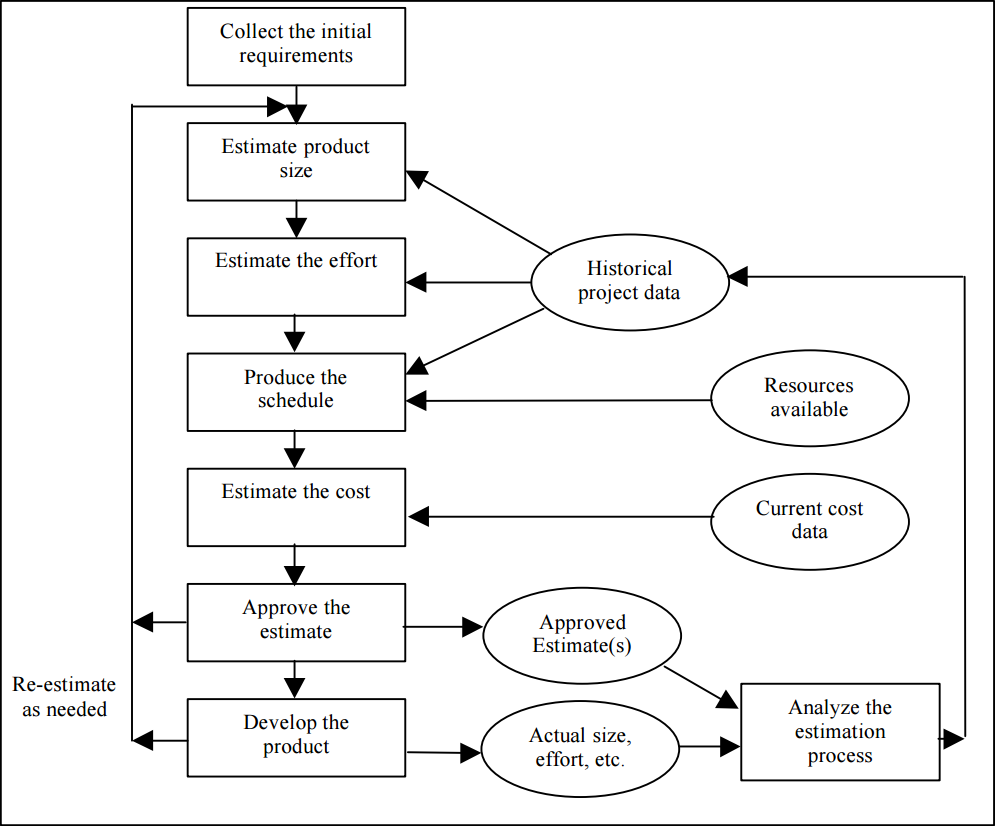
\includegraphics[width=13cm]{images/estimationProcess.PNG} 
	\caption{- The Basic Project Estimation Process}
	Source: Peters, Kathleen - Software Project Estimation, Page 3  
	\label{fig:basicEstimationProcess}
\end{figure}\\
In this classical view of the estimation process, it will generate four outputs - size (1.), loading (2.), duration (3.) and efforts (4.). The output can be described as following:
\begin{enumerate}
	\item Actual Size - the size of the project as a numerical value to make it comparable.
	\item Manpower Loading - the amount of personnel that is allocated to the project.
	\item Project Duration - the time that is needed to complete the project.
	\item Effort - the amount of effort required to complete the project is usually measured in units as man-days (MD) or person-months (PM).
\end{enumerate}
As described before, the estimation process can be triggered at any time in the project to re-estimate the costs. Depending on the project stage another estimation method than used before can be more precise.\\
The overview shown in \ref{fig:estimationMethodInStage} shows that the SLIM method, for example, is more suitable at the beginning of a project, whereas the ZKP method is more suitable after the system design stage. Most of the estimation methods can be used after the study stage. This is because after the study stage a rough overview of the project size exists. Different estimation methods may also change the evaluation output, which is one of the difficulties of cost estimations.\\
\begin{figure}[h] 
	\centering 
	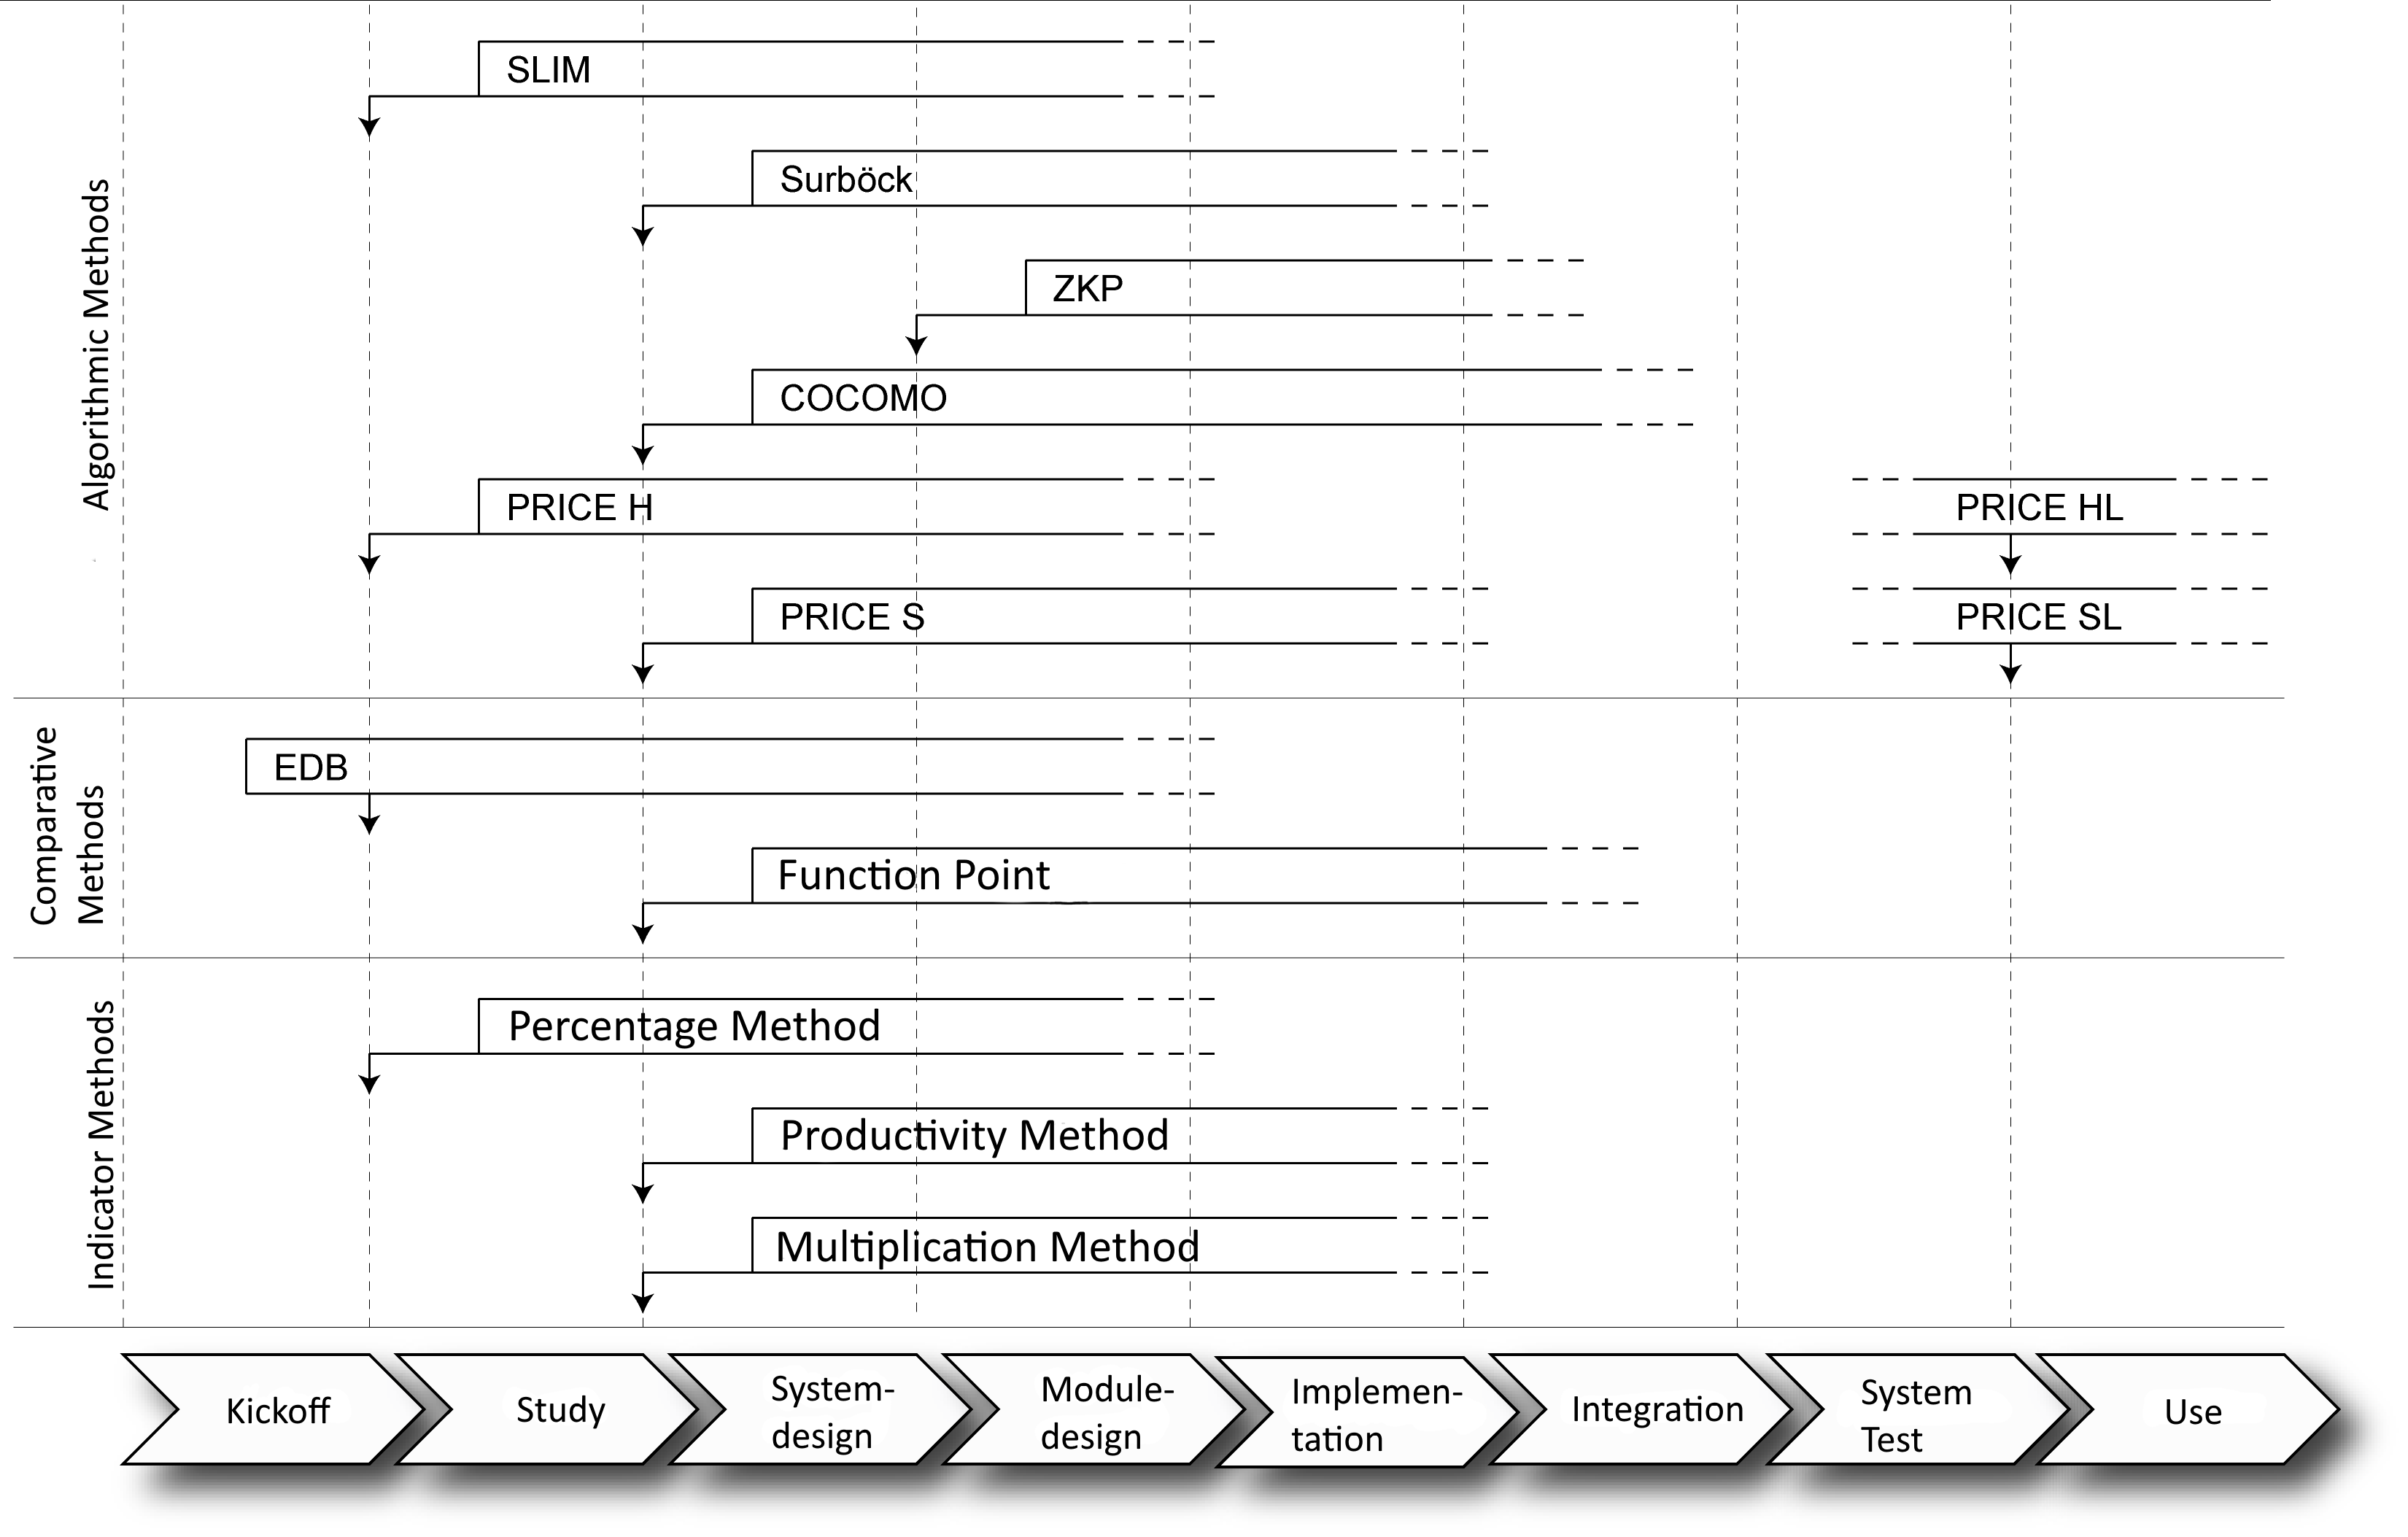
\includegraphics[width=13cm]{images/Einsatzzeitpunkte2.PNG} 
	\caption{- Starting Points of Estimation Methods} 
	Source: \url{http://winfwiki.wi-fom.de}
	\label{fig:estimationMethodInStage}
\end{figure}\\

\subsection{Difficulty of estimations}

One of the problems in estimating costs is that the actual code is only a small part of the project. Beside project planning there are many administrative tasks to do, like coordination of the project or searching and fixing errors. Most estimation methods evaluate the estimated time for the implementation and too little or no time is evaluated for the non implementation tasks. This resolves in an over- or underestimation of the non implementation tasks \cite{itplanung}.\\
Most project managers rely on their experience from past projects. This is an advantage, but as technology changes fast and new projects inherit new problems there is no prior experience for some parts of the project, what can make experiences from prior projects useless. Because of the unique nature of projects it is common that a new project has big parts where no experience exists. Another difficulty of estimations is the fact that people who are inherited in the project have a more positive outlook and mostly underestimate the costs.
Also, customers often got a target time for the project, which leads in adjustment of the cost estimation. This leads to budget overrun if the needed resources are not available for the project \cite{winfwiki}.\\
It is also not guaranteed that the estimated costs are accurate and stay within the budget. An estimation can easily go past their estimated target as new technologies and unexpected difficulties are commonplace. A partial requirements engineering can also cause an inaccurate cost estimation due to unexpected difficulties in the implementation. These this are different methodical approaches possible in which estimation methods can be classified, which is not described here.\\

\subsection{Methods for estimation}\label{chapter:estimationmethods}

Estimation methods are different metrics to calculate the costs of a project and there are different approaches to categorize the estimation methods. The categorization used in this paper is based on the book "Management von IT-Projekten" by Hans W. Wieczorrek, where the methods are subdivided in algorithmic, comparative, operating figures and expert discussion \cite{itplanung}.\\
All estimation techniques have in common, that only with a combined use of these different estimation methods a suitable result can be achieved as a measured value for the project. For the evaluation of the needed effort the underlying metric is used to calculate the effort for the project. On the basis of charge rates the effort size is calculated out of it.\\

\subsubsection{Algorithmic Method}

The algorithmic method uses a closed formula, which is based on empiric evaluation of already terminated projects or on existing mathematically models. Different forms of this method are the weight and the sampling method, which only differ in their usage.\\
The accuracy of the estimation depends primarily on the precision of the influence factors \cite{itplanung}. The algorithmic method always connects measurable project sizes, such as lines of code and implementable features, with influencing factors to get the result, represented as required effort in personnel costs. The basic formula, as described by Wieczorrek \cite{itplanung}, for this calculation is:

\begin{equation}
	Personnel costs = f(result quantity, influencing factors)
\end{equation}

\subsubsection{Comparative Method}

Not based on a formula or numerical connection, the comparative method tries to create a reference between the current project and past projects. Therefor projects from the own company or the same industry sector are analyzed with appropriate comparison methods. This estimation method has the advantage, that it can be used early in project development \cite{itplanung}. This method can be used for hardware and software projects.

\subsubsection{Key Figures Method}

Estimation methods based on key figures can be differed to multiplier and percentage  method. The multiplier method uses units of power as the base to estimate the total expenditure, whereas the percentage method uses the effort of a project stage to estimate the effort for the next stage.\\
After project completion a post calculation determines the total project costs and the amount of specific types of costs. In order to calculate these costs, they will be divided by the scope of the developed product. This results in new key figures which can be used for new projects by multiplication of the estimated scope with the appropriate key figures.\\
\cite{itplanung} Regular actualization of the key figures is necessary for right results.\\

\subsubsection{Expert Discussion Method}

As a quantitative, heuristic method the expert discussion uses knowledge from selected groups of people. It differentiates between four kinds: single person interview, multiple person interview, Delphi method and assessment meeting.\\
The advantage of this estimation method is, that they are useful for all project types. The problem with the expert discussion is, that this method is strongly affected by subjective opinions and the experience of the interviewees. As a result, expert discussions should never be used for complete projects but only for sub projects \cite{itplanung}.\\

\section{Estimation Techniques}

The existing estimation techniques rely on experience-based judgments by project managers
who created, by combining estimation methods, techniques can be used to estimate the effort of a project. Most of the estimation techniques became popular in the 80's, with the agile projects becoming more popular estimation techniques for these project types are rising. \\
Because of the fundamental uniqueness nature of projects an 'universal, everywhere applicable and always delivering the correct estimation' technique does not exist, according to Litke \cite{litke}. There is also no clear selection progress for the estimation technique to use, beside the time aspect when the use of a technique is possible. As shown in figure \ref{fig:estimationMethodInStage}, the function point and the COCOMO technique are both possible after the study stage. As a comparative method, the function point technique has not much in common with COCOMO, which is an algorithmic technique. The project manager has to balance the weigh of each technique and probably choose that one he has most experience with. As an example for estimation techniques these will be described here in more detail with a comparison at the end.


\subsection{Function Point} \label{FPMethod}

The Function Point technique was first mentioned by Allan J. Albrecht in 1979 at the IBM symposium \cite{albrecht}. There it was declared that an useful measurement of productivity is only possible in relation to the functionality that is visible to the user. This measured productivity needs to be independent of the used technology and is calculated in with the proportion of project effort and the allocated function points.\\
This resulted into the idea to turn this calculation over for a preliminary estimation of the effort the project would have. Because of to the clarity and flexibility the technique spread fast. It helps to estimate the scope of a project to an early stage and is suitable for benchmarking in the own company as well as on national or international level \cite{FPKompakt}. It contains algorithmic and also comparative methods. Basically, this technique uses five steps for estimation \cite{jenny}:
\begin{enumerate}
	\item Determining the components
	\item Evaluation of the components
	\item Calculating the function points
	\item Categorization of the influence factors
	\item Calculating the development effort with the function points and influence factors
\end{enumerate}
The most important part of this technique is that all measurements only include the user view. This means that the user view is focused on that functions that are important for the specific business process. Implemented business processes are the components that have to be determined.

\subsubsection{Determining the Components}

To divide the project in components that are useful for the function point estimation, all inherited business processes are divided into elementary process. These are the smallest and from business perspective view useful and closed activities, that can be performed by the system \cite{FPKompakt}.\\
A distinction is made into five categories:
\begin{enumerate}
	\item Input Data
	\item Output Data
	\item Request
	\item Dataset
	\item Reference Data
\end{enumerate}
It is useful to categorize the components, because a change in the datasets is followed by more effort than changing a request \cite{itplanung}.\\
The \textit{Input Data}, sometimes called \textit{External Inputs} (EI), is an elementary process in which data crosses the boundary from the outside of the application to the inside. This data comes from a data input screen or another application. To maintain one or more logical files, this data can be used for or to control business informations.\\
\textit{External Outputs} (EO), or Output Data, are an elementary process in which derived data passes across the boundary from the inside to the outside. Created output files or reports are sent to other applications. These are created from one or more internal logical files and external interface files.\\
Internal \textit{Logical Files} (ILF’s) or Dataset are an user identifiable group of logically related data that resides entirely within the applications boundary and is maintained through external inputs.\\
The next category are requests or \textit{External Inquiry} (EQ). An elementary process with both input and output components that result in data retrieval from one or more internal logical files and external interface files. This process does not update any Internal Logical files, and the output side does not contain derived data.\\
The last category is the \textit{Reference Data} or \textit{External Interface Files} (EIF), which are a user identifiable group of logically related data that is used for reference purposes only. This data resides entirely outside of the application and is maintained by another application \cite{fpafundamentals}.\\
After the categorization of the components there are for each category an amount of components, which then have to weighted for further evaluation.

\subsubsection{Evaluation of the Components}

The evaluation of the components is simply the classification of each category in their level of difficulty (simple, medium or complex). After this, each component is multiplied with the point value according to their difficulty. \\
The following table is described by Wieczorrek and are standard values for the function point technique \cite{fpafundamentals}:\\
\begin{table}[h] 
	\centering 
	\setlength{\tabcolsep}{4pt}
	\begin{tabular}{|l||c|c|c|}\hline
		Category & simple & medium & complex \\ \hline\hline
		Input Data & 3 & 4 & 6\\ \hline
		Output Data & 4 & 5 & 7\\ \hline
		Request & 3 & 4 & 6\\ \hline
		Dataset & 7 & 10 & 15\\ \hline
		Reference Data & 5 & 7 & 10\\ \hline
	\end{tabular}
	\caption{Point value of each category} 
	\label{tab:pointvalues} 
\end{table} \\

\subsubsection{ Calculating the amount of Function-Points}

After the evaluation there is an amount of components for each of the categories from above. To get the number of function points each category has to be multiplied according to the selected weigh and all categories are summed. This results in the following equation:

\begin{equation}
	E1 =  \sum \limits_{1}^n  (Function * Difficulty) \label{fp:E1}
\end{equation}

Function is the respective category and difficulty is the weigh from table \ref{tab:pointvalues}. The resulted value E1 is necessary for evaluating the estimated points with the influence factor.

\subsubsection{ Classification of Influence Factors}

Do get a more realistic estimation, all influences that can affect the project surroundings are measured. For the Function Point estimation there are seven defined influence factors \cite{Softwaremanagement}, which are described below.\\
Each of the influence factor has a value between zero and five which describes how much the factor influences the project.\\

\begin{enumerate}
	\item \textbf{Integration into other applications}\\The system will work with different applications and will send and receive data from other applications. This states if there is a cooperation with other applications and if the communication exists online or offline.
	\item \textbf{Local Data Processing}\\This factor describes if the system will work with distributed data. Zero means that the system does not work with other applications and five means that there is an integration into other applications in both ways.
	\item \textbf{Transaction Rate}\\A high transaction rate affects planing, development, installation and maintenance of the system. It describes how much transactions are to expected with the system.
	\item \textbf{Processing Logic}\\The processing logic can be divided in 4 subcategories: Arithmetic Operation, Control Procedure, Exception Regulation and Logic. Arithmetic Operation describes the intensity of the operations in the project. The controlling of the results stated within the Control Procedure influence multiplier. With the Exception Regulation it is described how eventual exceptions are treated and the Logic multiplier describes how much effort is to be expected for planning the logical component of the project.
	\item \textbf{Reusability}\\ How much of the produced software has to be reusable in other projects. A high value in reusability means extra effort in the planning stage for module-based development.
	\item \textbf{Stock Conversion}\\ This describes how much of the used data need to be transformed for the use within the project. A high value means much input from other applications that has to be transformed into data the application can process.
	\item \textbf{Facilitate Change}\\ The application was especially planned and developed in such a way that changes can be made easily. A high value means that the user can make changes on the system on its own and that the changes are available immediately.
\end{enumerate}
When all influence factors are set, all values for each factor will be summed up to the value E2. 

\begin{equation}
E2 =  \sum \limits_{1}^n   Influence Factor  \label{fp:E2}
\end{equation}\\
This influence factor indicator has then to be transformed to a multiplier that calculable with function points \cite{Softwaremanagement}\cite{fpafundamentals}.  

\begin{equation}
	E3 =\frac{E2}{100}  + 0,7 \label{fp:E3}
\end{equation}

\subsubsection{Calculation of the Function Points}

With the calculated Function Points (E1) and the Influence Factor multiplier (E3) are now the total-function-points (TFP) can be calculated with the following formula:
%equation,formula
\begin{equation}
	TFP = E1 * E3  \label{fp:TFP}
\end{equation}\\
From the regression analysis of previous projects a standard calculation of Function Points per day can be made with the table \ref{tab:pointsperday}.\\
The project has to be classified with their Total-Function-Points and divided through the appropriate points per day. The result of this calculation are the expected man days for this project.\\
\begin{table}[h] 
	\centering 
	\setlength{\tabcolsep}{4pt}
	\begin{tabular}{|l||c|c|}\hline
		Estimated Size    & Function Points & Points per Day\\ \hline\hline
		Small Project     & till 350        & 18 \\ \hline
		Mid Small Project & till 650        & 16 \\ \hline
		Medium Project    & till 1100 		& 14 \\ \hline
		Mid Large Project & till 2000 		& 12\\ \hline
		Large Project     & as of 2000 		& 10 \\ \hline
	\end{tabular}
	\caption{Function Points to Days} 
	\label{tab:pointsperday} 
\end{table} 

\subsection{COCOMO} \label{COCOMOMethod}

The Constructive Cost Model (COCOMO) is used when it is not possible to rely on experience. It is based on algorithmic and parametric methods, that merges parameters from software projects. Combining the system size, product properties, project and team factors with the effort for developing the system \cite{jenny}.\\
As an public domain model it is free to use and is considered to be a classic for algorithmic methods. It is common in many companies and is a technique which is adjusted to the IT development through the years.
The accuracy of the COCOMO techniques rises with later project stages. The deviation of the cost estimation is at the beginning of the project between \textit{0,25 * MD} and \textit{4 * MD}. In later project stages this variation decrease until it is zero just before the project ending \cite{sommerville}.\\
The parameters for COCOMO can be split into three parts. The project classes, model variants and the implementation time and effort.

\subsubsection{Project Classes}

The project classes represent the estimated size of the program itself. These are expressed in kilo delivered source instructions (KDSI). COCOMO classifies three project classes with different calculation factors as described in table \ref{tab:projectclasses} \cite{sommerville}.

\begin{table}[h]
	\centering 
	\setlength{\tabcolsep}{4pt}
	\begin{tabular}{|l||c|c|p{6cm}|}\hline
		Complexity	& Calculation Factor& KDSI 	& Describtion\\ \hline\hline
		Small   	& 1.05        		& $<$ 50  			& A small, well-known project team works together, the environment is well-known, there is no big innovation necessary and no pressure due to a deadline.\\ \hline
		Medium 		& 1.12        		& 50 - 300 			& Employees with average experience, team members with some experiences in subjections are working together.  \\ \hline
		Complex 	& 1.20 				& $>$ 300 			& High cost and deadline pressure, high innovations and an extensive project. High requirements to the project team and new components.  \\ \hline
	\end{tabular} 
	\caption{COCOMO project classes} 
	\label{tab:projectclasses} 
\end{table}

\subsubsection{Model Variants}

The COCOMO technique can be differed into the basis, intermediate and detailed variant. These represent the detail level of the cost estimation.\\
The first stage is also called basis estimation and is a rough estimation, which estimates the project costs to an early stage of the project. The costs are calculated with an equation without dividing the project into structure or time aspects. The base variant is an useful starting point for later estimations.\\
The second stage adjusts the first estimation to a higher level of detail by differentiating the development stages. It is not a parametric estimation yet, because not all data can be considered.\\
The detailed variant is the last stage of the estimation and allocate the estimation with fifteen in influence factors \cite{jenny}. These influence factors are divided into four categories. The product attributes inherit the required software reliability, the size of the application database and the complexity of the product. Run-time performance constraints, memory constraints, volatility of the virtual machine environment and the required turnabout time are members of the hardware attributes category. In the personal attributes are the influences analyst capability, software engineering capability. applications experience, virtual machine experience and programming language experience inherited. The last category is the project attributes which are described with the factors use of software tool, application of software engineering methods and required development schedule. Each of the 15 attributes receives a rating on a six-point scale that ranges from 'very low' to 'extra high' and have typical values in range from 0.9 to 1.4 .\\

\subsubsection{Calculation of Implementation Time and Effort}

Because of the differences in each variant of the COCOMO estimation, each variant has its own equation for calculation the costs. Each formula calculates the estimated time of the project in person-month (PM), which are stated by Boehm as 152 working hours resulting in one PM, with 19 working days and eight hour days \cite{boehm}. \\
The formula for the basic variant calculates the complexity of a project with the KDSI value and the calculation factor of the project which gives the calculated PM as a result. This formula is as follows:

\begin{equation}
PM = Complexity * (KDSI)^{Calculation Factor} \label{cocomo:basic}
\end{equation}\\
The KDSI value is the expected amount of code lines in the project and the Calculation Factor is the result of the table \ref{tab:projectclasses}. To figure out the complexity multiplicand the table \ref{cocomo:basicComplexity} describes for each project the suitable solution.\\
\begin{table}[h]
	\centering 
	\setlength{\tabcolsep}{4pt}
	\begin{tabular}{|l||c|}\hline
		Complexity	& Multiplicand\\ \hline\hline
		Small Project   	& 2.4        		\\ \hline
		Medium Project 		& 3.0        		\\ \hline
		Complex Project 	& 3.6 			\\ \hline
	\end{tabular} 
	\caption{COCOMO complexity multiplicands} 
	\label{cocomo:basicComplexity} 
\end{table}\\
The equation for the intermediate variant is the same as for the basic variant (\ref{cocomo:basic}). The difference is the changed multiplicand for this variant, as described in table \ref{cocomo:intermediateComplexity}.
\begin{table}[h]
	\centering 
	\setlength{\tabcolsep}{4pt}
	\begin{tabular}{|l||c|}\hline
		Complexity	& Multiplicand\\ \hline\hline
		Small Project   	& 3.2        		\\ \hline
		Medium Project 		& 3.0        		\\ \hline
		Complex Project 	& 2.8 			\\ \hline
	\end{tabular} 
	\caption{COCOMO complexity multiplicands} 
	\label{cocomo:intermediateComplexity} 
\end{table}\\

\subsection{Comparison}

adsf
a\\
a\\
a\\
a\\
a\\
a\\
a\\
a\\
a

\section{State of the art}

Vergleich welche Software es hierzu auf dem Markt gibt. Kurzbeschreibung der Software, Lizenzmodell, Kosten, Marktrelevanz
a\\
a\\
a\\
a\\
a\\
a\\
a\\
a\\
a

\subsection{The market}

Wieviele Softwareanbieter gibt es. Ist am Markt eine Nachfrage dafür. Gibt es mobile Anwendungen? Wird nach mobileren Anwendungen verlangt
a\\
a\\
a\\
a\\
a\\
a\\
a\\
a\\
a
\subsection{SEER - Cost Estimation Software}

The “Seer - Cost Estimation Software” is developed by Galorath Inc. in Los Angeles, USA. Galorath Inc. offers Consulting and Software for Cost Estimation, Decision Support and Project Management. The company was founded in 1979 with the goal to improve the software and hardware development process in the industry. The next step was to improve their consulting quality by developing their own tools for this process. Seer is the name of their toolset whit a large variety of how the different tools support the development process of new products.
\\
Seer for Software is an estimation application for "estimating, planning, analyzing and managing complex software projects" (galorath.com/products/software/SEER-Software-Cost-Estimation). Based on the SEER design principles the software contains an annotated and guided interface for defining projects, a parametric simulation engine and numerous standard and custom reporting options. Due to an open architecture API the SEER application can be integrated with enterprise applications and departmental productivity solutions. Galorath specifies that all estimations within this software are repeatable and consistent.
\\
According to the software description, "a high-level software estimate can be developed in a matter of minutes using SEER´s intuitive, window-based interface"(http://galorath.com/wp-content/uploads/2014/08/SEERforSoftware2.pdf). To start a new estimation a dialogue guides the user through the process. In the first screen the user has to set project name and decides whether he creates an empty project or starts with a scenario. The scenarios are example projects with some data for starting the estimation. In the next step the user choose the estimation method he wants to use for this project. The estimation methods are subdivided in functional, lines and sizing scale. Another feature of the software is the documentation and export function. All estimations can be exported to Microsoft Project, Microsoft Office, IBM Rational or other 3rd-party software. SEER delivers a huge variety of estimation methods, guided processes and many possibilities for documentation and reporting of all estimations.
\\
The software can be bought in an estimator, project manager and studio version. The estimator version inherits only standard estimation whereas the project manager and studio version allow estimation checking and access to the projects database. The studio version allows also independent crosscheck and verification. The price of each software version is nowhere specified.

\subsection{PRICE - Cost Estimation Software}

PRICE Systems L.L.C. provides agile and accurate estimating solutions. With their head office in Maunt Laurel, USA, and 12 locations worldwide they offer since 1969 estimating acquisitions. Their Software Development Cost Model is one of the oldest and most widely used software parametric models for software development projects. In 2003 PRICE released their Software TruePlanning, which contains methods that estimate the scope, cost, effort and schedule for software projects.
\\
For cost estimation, purchasing efficiency and budget planning PRICE Systems develops "multi-faceted cost estimating solutions" (http://www.pricesystems.com/en-us/leadership/priceoverview.aspx). Their biggest project is the PRICE Estimating Systems (ESI) Framework that delivers solutions for estimating projects and cost management. This framework is not specialized for estimating only software projects but also other projects.
\\
The integrated approach to Lifecycle Cost Management contains the PRICE Cost Estimation Framework. It is possible to estimate with all current state of the art cost estimations. The collaboration with other users is also possible as well as sharing the results through the program. This allows faster teamwork and a better estimation output. A data driven method for all estimations allows to compare the estimation with already completed projects. True Mapper allows also estimation output to a specific work breakdown structure or cost element structure for accurate top-down and bottom-up estimate comparisons. Mappings can be stored, retrieved, and modified to keep pace even as program activities change. Beyond specific cost estimating products and services, PRICE Systems offers strategic cost management services. They collaborate with estimators, engineers, project managers, and financial and executive management to design and implement integrated cost management systems that meet the unique challenges in the environment.
\\
There are not given any details about the cost of the software or licensing. This information must specifically enquire by Price Systems.

\subsection{SLIM Estimate}

SLIM Estimate is a cost estimating software developed by Quantity Software Management (QSM), an estimation company with their head office in McLean, USA. (http://qsma.com/slim-estimate/) QSM was founded in 1978 as a software management consultant company for measure, estimate and control projects. Beside their consulting business segment they develop the SLIM Software which contains software for controlling, metrics and estimation.
\\
The SLIM Estimate software provides a flexible cost estimation which align the estimation to the project size and new technologies. The estimation will hereby in the curse of the project enhanced. Integrated schedules offer simple exports of an existing calculation. The software can suggest alternate solutions calculated on past projects.
\\
The homepage got not into detail how this suggestion works. For a new estimating the user can use the SLIM Database and the QSMA knowledge. QSMA owns a huge database with past projects and industry standard estimation. This knowledge can be used for new estimations.
\\
For better use in the company the SLIM Estimate inherits interfaces to MS Office and the possibility export estimations as a web representation. SLIM Estimate delivers hereby a great software package with many functionalities. Especially the access to a large database and the knowledge base of QSM is a real added value to the application. As a result, it is possible in new projects to access the experience of past projects and get the benefit from this experience.


\subsection{Kinvey}

Kinvey is a software developer from Boston whose main business is the development of apps for business. In terms of cost estimates, the company is still very interesting. Since this company's mobile applications are developed individually for companies they need getting a cost estimate.
\\
Kinvey offers an online estimate for mobile applications with the potential customers can estimate the costs for their application. Here, the estimates are on the side of the cost and the length of time indicated by the customer would have to spend at a natural development, as well as the costs incurred for the customer if Kinvey developed the app for the company. The cost of developing through Kinvey here are always cheaper than a proprietary development.
\\
The cost estimation process is simple. The estimation schedule is a one-page where the user can select the components of his application. The user is guided through some question about features the application should contain. To answer these questions the user can either select one answer or more, which depends on the actual question. After each step the user can see the actual cost estimation of the project.
\\
The costs are calculated from the selected components in man days. It is possible to adapt in a further overview these cost estimates by hand again. It is not possible to define and add your own components for the estimation. The individual items that the user can choose are sorted by groups and displayed graphically. Estimating the cost of app development can also be used for your own estimates, but there is no way to export this estimation.

\subsection{Commonalities}

Was hat die Software gemeinsam, welche besonderen Features bei allen aufgefallen, wo ist ein feature das besonders heraussticht.\\
a\\
a\\
a\\
a\\
a\\
a\\
a\\
a\\
aa\\
a\\
a\\
a\\
a\\
a\\
a\\
a\\
a
\chapter{Application concept}

This chapter describes the project plan and the concepts for the developed application. These concepts are foundation of the developed application and describe how the internal processes in the application work.


\section{Project planning}

The project followed the incremental development model. For initial planning the features from existing cost estimation software as described in section \ref{sec:stateofart}. The next step was creating a \textit{GUI prototype} to show how the estimation would look like on a smartphone. Afterwards each cycle followed the rules of incremental development. An evaluation of the wanted features for the application was done in meetings with my supervisor Prof. Dr. Georg Rock. Those features request were compiled into the project goals and requirements. For the next step they were analyzed and implemented. Testing for the application were made afterwards by some of my fellow students. The result was then presented in a meeting and further features were planned for the next iteration cycle.
\begin{figure}[h] 
	\centering 
	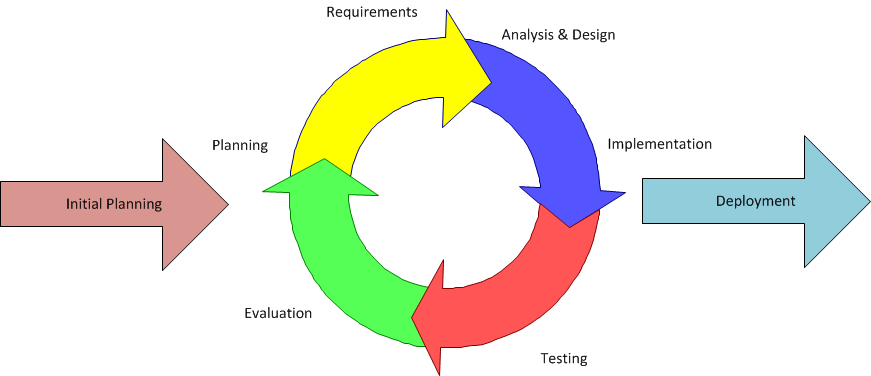
\includegraphics[width=14cm]{images/iterativeDev.PNG} 
	\caption{- Incremental Development} 
	Source: \url{https://www.inflectra.com/Methodologies/}
	\label{fig:incrementaldev}
\end{figure}\\


\subsection{Objectives}\label{objectives}

The project targets are the benefit the application should bring the user. They are linked with the requirements from section \ref{requirements} and describe the condition to be achieved with the application. Whereas requirements can change over time, targets stay the same.\\
Most important target, as described in table \ref{projecttargets}, is \textit{T01}. 'The application must allow a quick and mobile cost estimation of IT Projects' describes that the cost estimation has to be implemented for mobile device use. Also, the cost estimation has to be fast and can use features of the mobile platform to achieve this target.\\
As the developed application is only a beta version, it has to be developed modular for future feature implementation, as described in \textit{T04}.\\
\textit{T06} describes the target that represents an admired feature. The application should provide the possibility to compare projects and measure their relation. This allows to check previous projects for their cost estimation, that the user has a reference how much effort similar projects took.\\
The target for this bachelor thesis is to implement the function point estimation technique. This is the showcase for this application and shows the possibility of cost estimations for software project on mobile devices and is described in \textit{T09}.\\
All remaining targets are medium priority and describe what processes to achieve with this project.\\

\begin{table}[h]
	\centering 
	\setlength{\tabcolsep}{4pt}
	\begin{tabular}{|l||p{14cm}|}\hline
		ID		& Target\\ \hline\hline
		T01  	& The application must allow a quick and mobile cost estimation of IT Projects.\\ \hline
		T02  	& The application must provide informations how cost estimations work.\\ \hline
		T03  	& The application have to improve the cost estimation during  the project life cycle.\\ \hline
		T04  	& The application architecture has to be modular to add new cost estimation methods and analysis tools faster and more efficient.\\ \hline
		T05  	& With the application it is possible to get the information of completed projects and take advantage of their estimation.\\ \hline
		T06  	& The application allows comparison between projects and shows projects that are related to each other.\\ \hline
		T07  	& The application gives information about the estimated man days of a project and the estimated costs.\\ \hline
		T08  	& A project analysis within the application allows an overview of the project changes and gives detailed information about the estimation.\\ \hline
		T09  	& Till the end of the bachelor thesis the function point method has to be implemented and be fully operational.\\ \hline
	\end{tabular} 
	\caption{Project Targets} 
	\label{projecttargets} 
\end{table}

\subsection{Requirements}\label{requirements}

All requirements for the implemented application are based on the targets described in section \ref{objectives} and from the regular meetings. All requirements are described in the appendix XXXX and meet the demands for requirements as described by Balzert \cite{basiskonzepteRE}.\\


\subsection{Cost Estimation}
For the evaluation of the needed time, the project was estimated with the function point technique. Therefor all functionalities are grouped into functional groups, as described by Poensgen \cite{FPKompakt}. Afterwards each function was assigned a category for the estimation, as described in \ref{fpcomponents}.\\
The group Project, as described in \ref{fig:projectFunctionalityGroup}, inherits all functions for a project. All function groups for the application can be found in the application. The project functionalities in \ref{fig:projectFunctionalityGroup} are created with the requirements. Some requirements can be grouped into one functionality. As an example the function \textit{Create/Edit Project} inherits all requirements described in the appendix XXX. This function is marked as an \textit{EI} and \textit{ILF} because all changes are made by the user for this function and creates or edit all internal files for the project. \\
\begin{figure}[h] 
	\centering 
	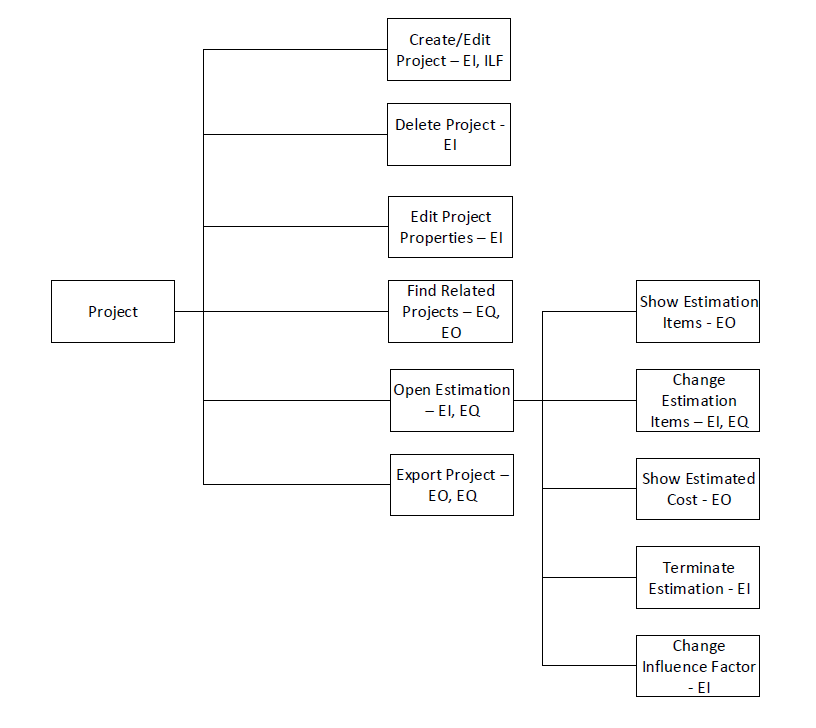
\includegraphics[width=14cm]{images/ScreenOverviewProject.PNG} 
	\caption{- Function Group - Project} 
	\label{fig:projectFunctionalityGroup}
\end{figure}\\
Functions that expects an input from the user are marked as \textit{EI}, like delete project. Output functions like show estimated cost are a \textit{EO} function, because they only display values and results to the user. Functions with a calculation are described as \textit{EQ} combined with \textit{EO} if they produce an output like \textit{Export Project} or process an \textit{Input} like \textit{Change Estimation}.The total functional group can be found in the appendix. This categorization of the function groups was inserted into the estimation table as described in table \ref{estimation:data}.Summed up the project has total \textbf{246} \textit{Function Points}.
\begin{table}[h]
	\centering 
	\setlength{\tabcolsep}{4pt}
	\begin{tabular}{|l|c|c|c|c|}\hline
		Category		&  Amount 		&  Classification	&  Weight 	& Sum of Row\\ \hline
		Input Data   	& 17      		& medium  			& 4			& 68	\\ \hline
		Request Data   	& 6      		& simple  			& 3			& 18	\\ \hline
		Output Data   	& 8      		& medium  			& 5			& 40	\\ \hline
		Dataset   		& 8      		& complex  			& 15		& 120	\\ \hline
		Reference Data  & 0      		& simple  			& 5			& 0	\\ \hline
		\textbf{Sum}   			&       		&   				& 			& \textbf{246}	\\ \hline
	\end{tabular} 
	\caption{Estimation - Total Points} 
	\label{estimation:data} 
\end{table}\\
As described in section \ref{FPMethod}, the next step is to set the influence factors which are described in table \ref{estimation:influence}. The influence factor \textit{Integration into other applications} is set to two because the application has no direct communication to other software. The application does not work with other applications but has local data, like the databases that have to be processed which is the reason for setting the factor \textit{Local Data Processing} to two. As the application is only a local software for the end users device their no much transaction to be excepted. To assure that there is enough time planned to implement a access to the database this factor is set to one. There are many algorithms and equations in the application which have to be checked for errors and exceptions. Also a high effort for the logical component is to be expected. Because of this all influence factors in the \textit{Processing Logic} group are set to the second highest value. For further development of the application a high effort has to be expected for \textit{Reusability} in the project which is the reason for this influence factor to be set at two. There is not much data to be expected from other applications. Only the database cause a higher effort with queries to transform the data from the database in readable informations for the application. Changes in the application can not be made by the user. He can change settings and some appearances which is why this influence factor is set to one. Completed with the equation from \ref{FPMethod} all influence factors result in a multiplier of \textbf{1.01}. Together with the total function points, the influence multiplier is calculated with the equation \ref{fp:TFP} which give \textbf{243.54} points as result. Calculated with the points per day from table \ref{tab:pointsperday} the project is estimated to take \textbf{14} man days. In section \ref{result} it is analyzed how this estimation has worked out and how much time the project took.\\
\begin{table}[h]
	\centering 
	\setlength{\tabcolsep}{4pt}
	\begin{tabular}{|l|c|}\hline
		Influence Factor						&  Weight 	\\ \hline
		Integration into other applications   	& 2      		\\ \hline
		Local Data Processing   				& 2      		\\ \hline
		Transaction Rate   						& 1      		\\ \hline
		Processing Logic   						&       		\\ \hline
		\phantom{ab}- Arithmetic Operation   					& 4      		\\ \hline
		\phantom{ab}- Control Procedure   					& 4      		\\ \hline
		\phantom{ab}- Exception Regulation   					& 8      		\\ \hline
		\phantom{ab}- Logic   								& 4      		\\ \hline
		Reusability   							& 3      		\\ \hline
		Stock Conversion  						& 2      		\\ \hline
		Facilitate Change   					& 1      		\\ \hline
		\textbf{Sum}   									& \textbf{31}      		\\ \hline
	\end{tabular} 
	\caption{Estimation - Influence Factors} 
	\label{estimation:influence} 
\end{table}

\section{Architecture}

The architecture of the project is described as a component diagram in fig. \ref{fig:components}. As usual in Android developments all resources are stored in the \textit{resources} folder and are accessible from all other classes. The resources inherits \textit{strings}, \textit{images} and many more. Most used in the same folder is the \textit{Layout Data} which inherits all informations for displaying the user interface. Layout informations are connected with the \textit{Activities} and \textit{Fragments} component which are responsible to display the user interface.\\
The \textit{Project Analyzer} component is responsible for collecting the data from all projects and put them together for analysis. As the name says, \textit{Project Data} contains all informations for a single project. For reading and storing data to the database the component \textit{Database Helper} is the part that allows simple \textit{Data Requests} and \textit{Data Insertions} to the database. It also allows a connection to the \textit{XML Helper} which reads data that is stored to XML files. The

\begin{figure}[h] 
	\centering 
	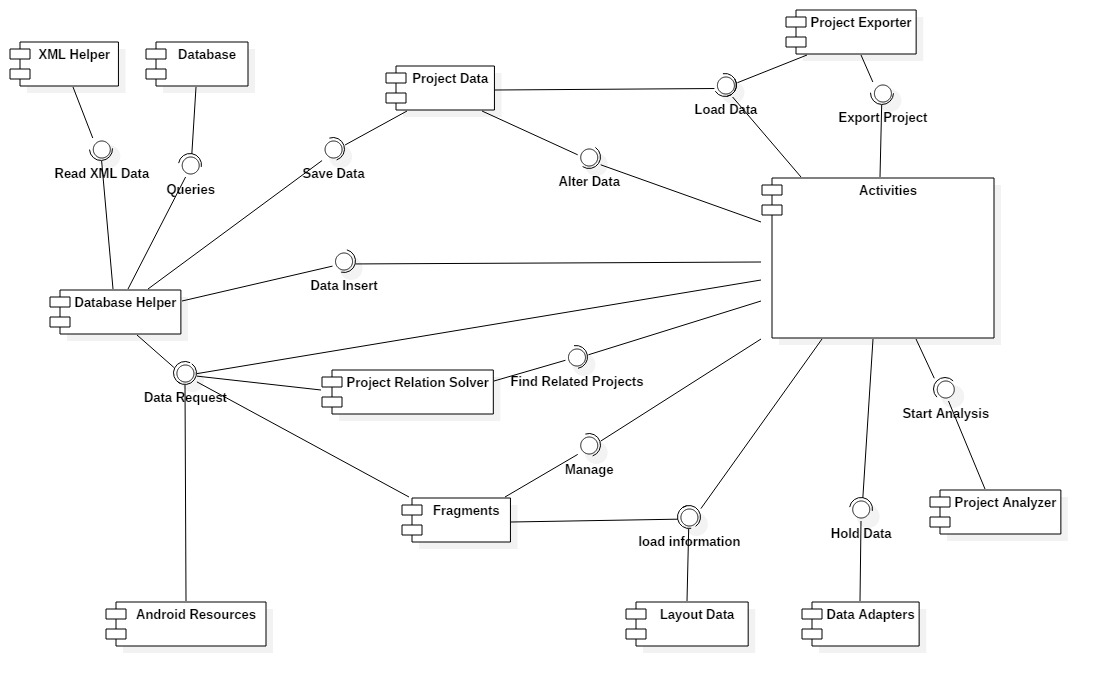
\includegraphics[width=14cm]{images/components.jpg} 
	\caption{- Component Diagram} 
	\label{fig:components}
\end{figure}

\section{Components}

This section describes the most important components from figure \ref{fig:components} in detail and what concepts they inherit. 

\subsection{Database Helper}

The \textit{Database Helper} component is responsible for accessing the database, where all project informations are stored. Every Class that needs access to the database should only create an object of this component and can read or write data to the database.\\
The component should contain name and path to the database and allow the initialization of the database. As described in fig. \ref{fig:sequenceDBHelper}, with the message \textit{Open Constructor}, an initialization of the database should be done in the constructor of classes that need access to it. This will opens the \textit{SQLite} database and ensures that request on the database can be performed and no error occurs while accessing a non initialized database. All functionalities that are working on the database are in fig. \ref{fig:sequenceDBHelper} combined to the message \textit{Using Class} and combines the three categories for working with the database \textit{SELECT}, \textit{ALTER} and \textit{DELETE}.\\ 
For requesting data from the database a Java class has to send a request with the table name and the selection criteria to the Database Helper. This will be transformed into a query which is send to the database. Before sending this data back to the calling Java class the database Helper has to transform the \textit{SQL} query result into readable information. Editing existing informations in the database is done with the message \textit{Alter Existing Data} and the parameters table name and data to be edited. Before sending data to the database the \textit{Database Helper} has to prepare it to insert them in the right column of the table. This query will return true if inserting was successful or false if it was not. Last message option is \textit{Delete Data} which will delete entries from the database. The parameter \textit{tablename} and \textit{Data ID} are the identifiers for a selected entry. Before deleting data from the database the \textit{Database Helper} has to check if there are any other tables depending to the selected entry and have to ensure that they are deleted too if necessary. After all depending tables are identified the Database Helper will send the delete query to the database. It will then return a boolean value for the deletion process which is forwarded to the Java Class.

\begin{figure}[h] 
	\centering 
	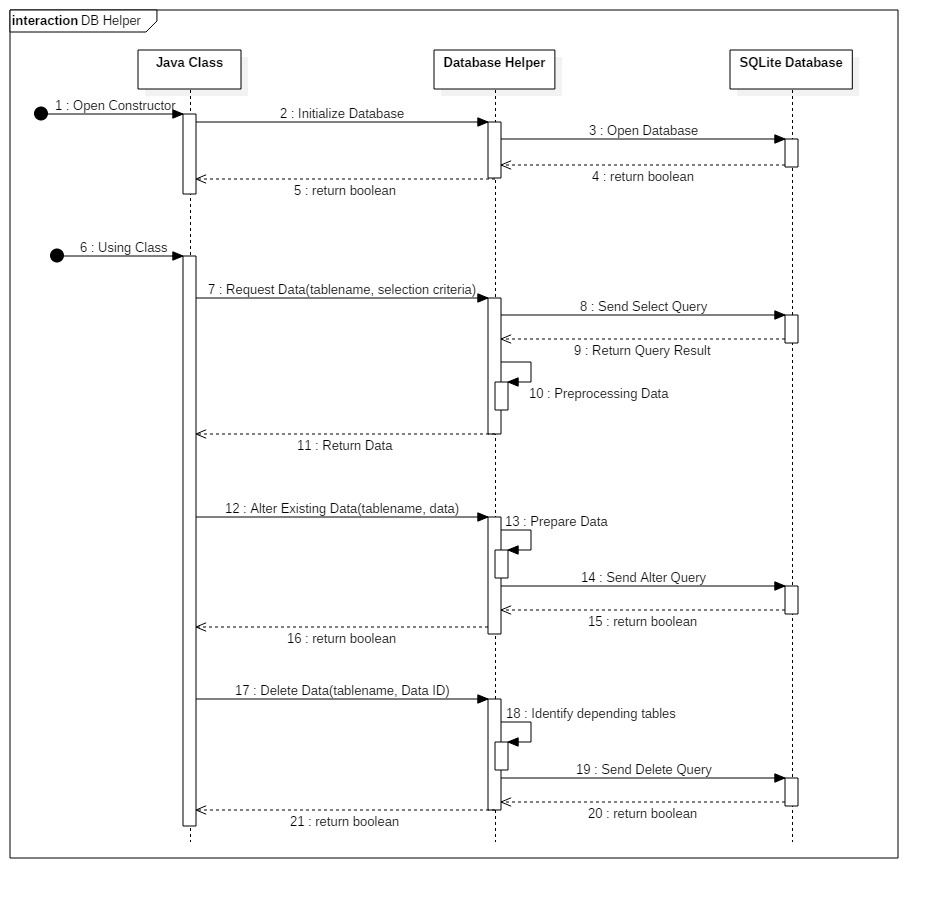
\includegraphics[width=14cm]{images/DBHelper.jpg} 
	\caption{- DB Helper Sequence Model} 
	\label{fig:sequenceDBHelper}
\end{figure}

\subsection{Project Data}

The \textit{Project Data} component was created to make combine all data of a project from the database and make it accessible for other classes. It contains \textit{Name}, \textit{Description}, \textit{Creation Date} and \textit{Estimation Technique} at the first level of the component. This makes it possible to get a fast overview of the different projects in the application. For estimation specific purposes the \textit{Estimation Items} and \textit{Influence Factor} are minor components for the project data and differ from the projects estimation technique. The \textit{Properties} are also a minor component to build a module-based structure. As the output information of estimation techniques is the same, the main component contains the amount of \textit{Estimated Man Days} for the project. If the project is completed the \textit{Final Man Days} represent the time the project really took. This value is important to improve future estimations as described in section \ref{adjustedEstimationProcess}, where the improvement process is specified.
\begin{figure}[h] 
	\centering 
	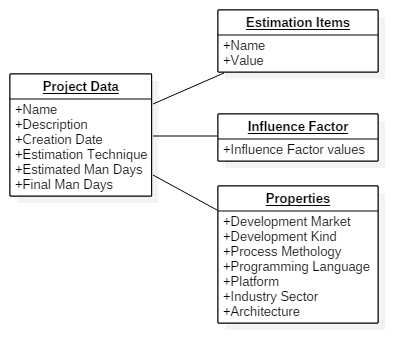
\includegraphics[width=10cm]{images/ObjectDiagramProject.png} 
	\caption{- Object Diagram for Projects} 
	\label{fig:objectDiagrammProject}
\end{figure}

\subsubsection{Project Properties}

This minor component contains the information that is needed for the \textit{Project Relation Solver} in section \ref{projectRealtionSolver}. It is a data component which stores all properties that allows reading and editing. Access to is granted to the properties only through the project component which assures that a property is bound to a project.\\
The available properties are based upon the parts a project can be split to. Not every available factor of a project makes sense for categorizing it. For example a categorization into the size of the project makes no sense as this cannot be compared to a project that is not estimated or developed. Although a categorization in the costs makes no sense as it cannot be compared to a project that has to be estimated. For this reason the available properties are \textit{Development Market}, \textit{Development Type}, \textit{Procedure Model}, \textit{Platform}, \textit{Industry Sector}, \textit{Programming Language} and \textit{Software Architecture}. These values categorize a project without saying something about the size or cost and make it possible to compare them.\\
All project properties contain only a selection of the possible values as a showcase. For each category are further options possible. For properties where this is a important factor these are combined in the option \textit{other}.\\
\subsubsection{Estimation Items}

All items for the estimation are in the \textit{Estimation Items} components. These are the items for an estimation technique that are responsible for the estimation itself. In the \textit{Function Point} estimation for example, these items calculate the value \textit{E1} from the equation \ref{fp:E1}.\\

\subsubsection{Influence Factors}

This component contains all informations for \textit{Influence Factors}. These are \textit{name}, \textit{chosen value} and the \textit{limit} for the value. This component is also responsible for preprocessing the influence factor for usable information at the calculation of the estimation. In the Function Point estimation for example, this component calculated the value \textit{E2} and \textit{E3} that are described in section \ref{fp:classificationInfluence}.\\

\subsection{Project Relation Solver}\label{projectRealtionSolver}

To fulfill the target \textit{T06} from section \ref{objectives}, this component is responsible to find related project. The point of this component is to compare already existing projects with a selected one. This should help the user to get an overview of how similar projects were estimated. Furthermore the \textit{Project Relation Solver} should allow to transfer the estimation from a related project to the selected to have an estimation where the user can build on.\\
The \textit{Project Relation Solver} compares therefor an selected project with every other available project from the database. This comparison is made in mainly three steps.
\paragraph*{\textbf{1. Determination of the Property Distances}}
Each project has seven different properties which are crucial for finding a relation plus the estimation technique. These properties are \textit{Development Market}, \textit{Development Kind}, \textit{Procedure Model}, \textit{Platform}, \textit{Industry Sector}, \textit{Programming Language} and \textit{Software Architecture}. The first step for calculating the project relation is to compare each property and get the distance. Each of them has its own calculation for the distance and a different weight to fit in the \textit{total distance} equation. 
\paragraph*{\textbf{Development Market}}
The \textit{Development Market} property stands for the target market of a project and has three possible options: \textit{Inhouse Development}, \textit{Customer Development} and the \textit{Anonymous Market}. For calculating the distance between development markets it was analyzed for whom the project is developed, what is the main factor for the budget, how high is the risk of development and how predictable profit is.\\ 
The \textit{Inhouse Development} is a for developing projects in the company. They are usually have the same procedure as other project despite the fact that they don't yield a profit and have a low risk of development and a fixed budget. In the \textit{Customer Development} the risk depends on the customer needs but are predictable. Profit is to be expected high and is connected with the project budget. By \textit{Anonymous Market} developments a high risk is to be expected. Regardless of market analysis it is unsure that the project will be a success and generate profit. The budget for this market type is set from the company itself.\\
All distances between these markets are described in table \ref{property:devmarket} and are based on the above description. For example, the development for a customer is quite similar to an anonymous market development the distance between those is set to one. The big difference is that the profit is unsure for the anonymous market development. When comparing similar markets to each other the distance is zero as they are the same.
\begin{table}[h]
	\centering 
	\setlength{\tabcolsep}{4pt}
	\begin{tabular}{|l|l|c|}\hline
		Development Market		& Compared to 			&  Distance 	\\ \hline
		Inhouse Development   	& Customer Development	& 2      		\\ \hline
		Customer Development   	& Anonymous Market 		& 1      		\\ \hline
		Anonymous Market   		& Inhouse Development 	& 3     		\\ \hline
	\end{tabular} 
	\caption{Development Market - Distance} 
	\label{property:devmarket} 
\end{table}
\paragraph*{\textbf{Development Type}}
Different \textit{Development Types} describe the main reason for the project. A \textit{New Project} is developed if there is no previous project to build on or is a new conceptual formulation. An \textit{Extension Project} is made for expansion of existing software from previous projects. The third type are \textit{Research Projects} which are usually made to test an idea or create a prototype for an analysis. These development types can be differentiated in the \textit{main target} of the project, \textit{customer} and \textit{profit level}. To introduce this differentiation the profit level describes the expected money and is divided into values from zero to two. \textit{Zero} declines that the project does not generate any profit. The value \textit{one} expects medium profit and \textit{two} expects a high profit for the project.\\
The distances described in table \ref{property:devtype} are based on the above descriptions. A comparison between new projects and research project has the distance two. A research project does not generate any profit and has a different target than a new project. The same applies with the comparison of an extension project with a research project. By comparing a new project to an extension project the distance is set to one because the expected profit is smaller than in a new project. The reason for this is that an extension project builds up on a previous project and is an addition to a previous contract which normally get a smaller budget.\\
\begin{table}[h]
	\centering 
	\setlength{\tabcolsep}{4pt}
	\begin{tabular}{|l|l|c|}\hline
		Development Type		& Compared to 			&  Distance 	\\ \hline
		New Project   			& Research Project		& 2      		\\ \hline
		Extension Project   	& New Project 			& 1      		\\ \hline
		Research Project   		& Extension Project 	& 2     		\\ \hline
	\end{tabular} 
	\caption{Development Market - Distance} 
	\label{property:devtype} 
\end{table}
\paragraph*{\textbf{Procedure Model}}
The next property is the used procedure model. There are six procedure models for selection available. The distance in table \ref{property:proceduremodel} is calculated by differentiating each procedure by model type, suitable team size, formalization, industry focus and process cover. Model type simply splits the procedure models in sequential and iterative types. The suitable team size indicates the laid out size of team members are useful for this model. Formalization indicates how much has to be put into the documentation of the process steps and the process cover describes if the procedure model involves all main project processes which are development, test project management, quality assurance and the change management.
\begin{table}[h]
	\centering 
	\setlength{\tabcolsep}{4pt}
	\begin{tabular}{|l|l|c|}\hline
		Procedure Model			& Compared to 	&  Distance 	\\ \hline
		Scrum   				& V-Model		& 5      		\\ \hline
		Waterfall Model   		& V-Model 		& 3      		\\ \hline
		Spiral Model   			& V-Model 		& 4     		\\ \hline
		Iterative Development   & V-Model 		& 4     		\\ \hline
		Prototyping  			& V-Model 		& 6     		\\ \hline
	\end{tabular} 
	\caption{Procedure Model - Distance} 
	\label{property:proceduremodel} 
\end{table}

\paragraph*{\textbf{Platform}}
Platform is the property that describes where the implemented software is deployed. The difference between platforms is calculated with the porting costs from one platform to another. This costs are calculated with the main programming language of the platform, quality assurance, system type and the deployment difficulty.\\
\begin{table}[h]
	\centering 
	\setlength{\tabcolsep}{4pt}
	\begin{tabular}{|l|l|c|}\hline
		Platform			& Porting to 	&  Costs 	\\ \hline
		Android   			& IOS					& 3      		\\ \hline
		Android   			& Windows Phone 		& 3      		\\ \hline
		Android   			& Mac OS 				& 5     		\\ \hline
		Android   			& Linux 				& 4     		\\ \hline
		Android  			& Windows 7 			& 5     		\\ \hline
		Android  			& Windows 8				& 5     		\\ \hline
		Android  			& Windows 10 			& 5     		\\ \hline
		Android  			& Windows Universal App	& 6     		\\ \hline
		Android  			& Web Development 		& 5     		\\ \hline
		Android  			& Other 				& 7     		\\ \hline
	\end{tabular} 
	\caption{Platform - Porting cost} 
	\label{property:platform} 
\end{table}\newpage

\paragraph*{\textbf{Industry Sector}}
For the industry sector there is no calculated distance as it is mostly an empiric property. It simply compared if the selected sectors are equal or not. If the industry sector does not apply to one of the available sectors there is the option to select \textit{Other} as sector. For the calculation the distance between industry sectors is set to \textit{zero} if they are equal and  \textit{one} otherwise. The available options for this property are:
\begin{itemize}
	\item \textit{Agriculture}
	\item \textit{Automotive}
	\item \textit{Banking}
	\item \textit{Bars and Restaurants}
	\item \textit{Business Service}
	\item \textit{Construction}
	\item \textit{Education}
	\item \textit{Electronics}
	\item \textit{Entertainment}
	\item \textit{Finance}
	\item \textit{Health}
	\item \textit{Internet}
	\item \textit{Music Production}
\end{itemize}

\paragraph*{\textbf{Programming Language}}
The Programming Language describes the main language for the project. As an example for the platform Android the main programming language would be Java. This Property has the most values for calculating the distance between two options. It is divided in two parts. Part one is calculating distance on the basis of programming language properties as described by Ruknet \cite{ruknet}. He categorized the programming languages with 12 different properties:
\begin{enumerate}
	\item \textbf{Imperative}\\ This value focuses in describing how a program operates. It simply exists on a sequence of instruction. This value is distinguished with \textit{true} or \textit{false}.
	\item \textbf{Object Oriented}\\ This Property describes if the language supports the concept of objects.
	\item \textbf{Functional}\\ These property is a programming paradigm that treats computation as the evaluation of mathematical functions. 
	\item \textbf{Procedural}\\ This programming paradigm allows routines and subroutines and contains a series of computational steps.
	\item \textbf{Generic}\\ Generic programming is a style which allows algorithms to be written in terms of types \textit{to-be-specified-later} that are then \textit{instantiated} when they are needed.
	\item \textbf{Reflective}\\ This is the ability of a programming language to examine and modify its own structure and behavior.
	\item \textbf{Event-Driven}\\ An event-driven programming language is determined by events such as user actions or messages from other programs.
	\item \textbf{Failsafe}\\ The ability to throw exceptions if an operation or other system calls fails is known as fail safely.
	\item \textbf{Type Safety}\\States if a programming language discourages or prevents type errors which are stated in the values \textit{safe} or \textit{unsafe}
	\item \textbf{Type Expression}\\ This property describes if the programmer must explicitly associate each variable with a particular type.
	\item \textbf{Type Compatibility}\\ This implies the use of a type checker in the programming language which verifies if an expression is consistent with the expected type by the context in which that expression appears.
	\item \textbf{Type Checking}\\ A process of verifying and enforcing the constraints of types.\\
\end{enumerate}
Each property is converted to a numerical representation form which represents each of the possible values. This allows a calculation of the \textit{Distance} of two programming languages. As described in equation \ref{pl:distanceequation} this calculated with the absolute value of each category. The constant \textit{c} is the amount of all categories, which is twelve. For each category \textit{$K_i$} of the compared programming language the value of the other language is subtracted. This summed up is the distance of these two languages.
\begin{equation}
\textit{Distance} = \sum \limits_{i=1}^c \lvert K_i - K'_i\rvert \label{pl:distanceequation}
\end{equation}
\begin{table}[h]
	\centering 
	\setlength{\tabcolsep}{4pt}
	\begin{tabular}{|l|c|c|c|c|c|c|c|c|c|c|c|c|}
		\multicolumn{1}{c}{\textbf{Programming Language}}& \multicolumn{1}{c}{\rotatebox{90}{imperative} }&  \multicolumn{1}{c}{\rotatebox{90}{object oriented}} &  \multicolumn{1}{c}{\rotatebox{90}{functional}}&  \multicolumn{1}{c}{\rotatebox{90}{procedural}}& \multicolumn{1}{c}{\rotatebox{90}{generic}}&  \multicolumn{1}{c}{\rotatebox{90}{reflective}}& \multicolumn{1}{c}{\rotatebox{90}{event driven}}&  \multicolumn{1}{c}{\rotatebox{90}{failsafe}}&  \multicolumn{1}{c}{\rotatebox{90}{type safety}}&  \multicolumn{1}{c}{\rotatebox{90}{type expression}}&  \multicolumn{1}{c}{\rotatebox{90}{type completion}}&  \multicolumn{1}{c}{\rotatebox{90}{type checking}}\\ \hline
		C++   				& 1& 1 & 1 & 1& 1& 0& 0& 0& 1& 2& 1& 0    		\\ \hline
		Java   				& 1& 1 & 1 & 1& 1& 1& 0& 2& 1& 2& 1& 1    		\\ \hline
	\end{tabular} 
	\caption{Programming Language - Distance} 
	\label{property:proglang} 
\end{table}

The second part is the conversion cost in another language which is the estimated effort for converting the source code. For calculating these \textit{Conversion Costs} the equation \ref{pl:conversioncosts} delivers an estimated cost factor. These costs are simply the \textit{Amount} of different categories plus an constant effort factor of one.


\begin{equation}
\textit{Conversion Costs} = \textit{Amount} + 1\label{pl:conversioncosts}
\end{equation}

The available languages are C, C\#, C++, COBOL, Clojure, Java, Javascript, Matlab, Objective-C, PHP, Prolog, Python and Scala. The complete categorization and converting costs of all programming languages can be found in the appendix XXX.


\begin{table}[h]
	\centering 
	\setlength{\tabcolsep}{4pt}
	\begin{tabular}{|l|l|c|}\hline
		Programming Language	& Converting to &  Distance 	\\ \hline
		Java   				& Cpp		& 4      		\\ \hline
	\end{tabular} 
	\caption{Programming Language - Conversion Cost} 
	\label{property:proglangconversion} 
\end{table}

\paragraph*{\textbf{Software Architecture}}
asd
\begin{table}[h]
	\centering 
	\setlength{\tabcolsep}{4pt}
	\begin{tabular}{|l|c|c|c|c|c|c|c|}
		\multicolumn{1}{c}{\textbf{Software Architecture}}& \multicolumn{1}{c}{Category }&  \multicolumn{1}{c}{\rotatebox{90}{overall agility}} &  \multicolumn{1}{c}{\rotatebox{90}{ease of deployment}}&  \multicolumn{1}{c}{\rotatebox{90}{testability}}& \multicolumn{1}{c}{\rotatebox{90}{performance}}&  \multicolumn{1}{c}{\rotatebox{90}{scalability}}& \multicolumn{1}{c}{\rotatebox{90}{ease of development}}\\ \hline
		Client-Server   	& interactive& 2& 1 & 3& 3& 3& 2   		\\ \hline
		MVC   				& distributed& 2& 3 & 2& 3& 3& 2    		\\ \hline
	\end{tabular} 
	\caption{Software Architecture - Distance} 
	\label{property:architecture} 
\end{table}

\paragraph*{\textbf{2. Determination of the Total Distance}}
asdasdasd
\paragraph*{\textbf{3. Calculation of the Relation}}
asdasdasd\\
asdasd

\subsection{Project Analyzer}

Aufbau der Analyze der Projekte, Wie die Graphen vorgestellt. Sinn davon

\subsection{Minor Components}

Export, statistic, Help DB, Feedback, Project Filter, accessing resources


\section{Database design}

Vorheriges Design der zentralen Datenbank. Wichtig um die Klassen anzupassen und vorher schon mit wichtigen Daten zu füllen

\subsection{Project Database}

Datenbank für alle Projekte, Eigenschaften, Einflussfaktoren

\subsubsection{Project Properties}

Welche Tabellen gibt es. Wichtige Tabellen, Aufbau der Tabellen und Grund

\subsubsection{Influence Factors}

Wie die Einflussfaktoren Aufgebaut, was ist der Gedanke dazu?

\subsubsection{Projects}

Wie sind Projekte gespeichert, Aufteilung in Projekt, Projektdetails und zugehörige Tabellen, wie die Schätzung Organisiert und wie der Zugriff auf die Elemente

\subsection{Userinformation Database}

Datenbank für Spätere Synchronisation und Userinformationen vom Server, Konzept dazu

\section{User Interface}

\subsection{Projects Overview}

Anordnung der Projekte, Wichtige Informationen zum sehen, Filtern und Suchen nach Projekten

\subsection{Project Creation}

Komponente zur korrekten Erstellung von Projekten, Geführte Eingabe, Korrekte Erstellung von Projekten in der DB, Swipe Funktion

\subsection{Estimate Function Point Project}

Aufbau der Schätzung, Umwandlung von Tabelle in App

\subsection{Influence Factors}

Aufbau der EInflussfaktoren, Neue anlengen

\subsection{Analysis}

Wie die Analyse aufgebau und was soll diese bringen?

\section{Adjusted Estimation Process}\label{adjustedEstimationProcess}


\subsection{Continuous Improvement of the Estimation}


\chapter{Implementation}

The used libraries and selected implementation approaches are described in this chapter. \textit{Android Studio} was used as the \textit{IDE} for development and \textit{GitHub} was used for version management. 

\section{Used Libraries}

For the implementation were two external libraries necessary. These libraries are called \textit{POI} and \textit{mpandroidchartlibrary}. \textit{POI} is a library from the \textit{APACHE Software Foundation} and is open source. It allows a conversion of data into Microsoft documents. This library is used
in the \textit{Export} component and allows to create \texttt{xls} documents with the project data. The \textit{mpandroidchartlibrary} library is also an open source library developed by Philipp Jahoda. This library provides many different diagram types for Android such as pie and bar charts. This charts are used for the estimation technique analysis and for the project statistics. 

\section{Project Structure}

Android divides the project into an \textit{assets}, \textit{resources} and \textit{java} folder. The \textit{assets} folder stores project icons and the two databases of the project. After installation of the \texttt{apk}, these files are moved to the internal folder space of the application. The \textit{resources} folder contains every \texttt{layout} file, \texttt{string} resources and the android \texttt{icons}. All resource files ar typically \texttt{XML} files or in case of images \texttt{png} files. The \textit{java} folder contains the complete source code. This folder was divided into the sub folders \textit{Activities}, \textit{Fragments}, \textit{DataObjects}, \textit{Server} and \textit{Util}. The folders \textit{Activities} and \textit{Fragments} contain the associated classes for each layout and are responsible to control the user input. In the folder \textit{DataObject} are all data classes stored. These are objects that only store data and don't have any logical components. The \textit{Server} folder contains at the moment only the \texttt{ServerConnector} class. This folder was created to separate the future server connection. Last folder is the \textit{Util} folder. It contains classes that process data, for example the \texttt{DatabaseHelper} class.

\section{Pre-filled Database}\label{exDB}

The advantage of a pre-filled database is a shorter initialization after first start of the application. The database doesn't have to run many \textit{SQL} scripts to create tables and insert values. Also values and tables can be created with an external tool such as \textit{SqliteBrowser}\footnote{\url{http://sqlitebrowser.org/}}. This allows testing of the tables and \textit{queries} that are used in the application. To use this database two steps are essential:
\begin{enumerate}
	\item \textbf{Create Database}
	\item \textbf{Open Database}
\end{enumerate}
Both methods are inherited in the class \texttt{DataBaseHelper}. Listing \ref{createdb} shows the method \texttt{createDataBase()} which is responsible for the creation of the database. At first the method checks with \texttt{checkDataBase()} if the database does already exist in the \texttt{application} folder. If it does not exist the method calls \texttt{copyDatabase()} which will read the database from the \texttt{assets} folder and write a new database to the application folder.
\begin{lstlisting} [caption=Method \textit{createDataBase}, label=createdb] 
public void createDataBase() throws IOException
{
	boolean dbExist = checkDataBase();
	if (!dbExist)
	{
		this.getReadableDatabase();
		try
		{
			copyDataBase();
		} catch (IOException e)
		{
			Log.d("ERROR", "Database could not be copied " + e.getCause());
			throw new Error("Database could not be copied");
		}
	}
}
\end{lstlisting}
Open the database is done with the method \texttt{openDataBase()}, which is described in listing \ref{opendb}. The class variable \texttt{projectEstimationDataBase} is initialized here with the \texttt{SQLiteDatabase} command \texttt{openDatabase} which create a \texttt{SQLiteDatabase} object with the path where it is stored. This allows the execution of \texttt{SQL} queries in this object.
\begin{lstlisting} [caption=Method \textit{openDataBase}, label=opendb] 
public void openDataBase() throws SQLException
{
	String myPath = DB_PATH + DB_NAME;
	projectEstimationDataBase = SQLiteDatabase.openDatabase(myPath, null,
										 SQLiteDatabase.OPEN_READWRITE);
}
\end{lstlisting}
\section{The Database Helper}

The \texttt{DataBaseHelper} class has the most lines of code in the project. As \texttt{SQL} queries can be generalized it is not possible to generalize the preprocessing of the data. Different date needs different treatment for the calling method. Each table has also various column names what is another difficulty for generalization. \\
All requests with \texttt{SELECT} statements have a similar structure. As described in listing \ref{selectStatement}, the first step is to build a \texttt{String query} with the table name and parameter from the method. Next step is to get a readable database from the \texttt{SQLiteDatabase} object of this class. The query will be executed on this object and creates a \texttt{Cursor}, which is the result table. To get the values from this \texttt{Cursor} each column has to be addressed and saved into a variable which will be returned to the caller. If more values are needed those have to be packed into other data structures.
\begin{lstlisting} [caption=Method \textit{openDataBase}, label=selectStatement] 
public void selectSomethingFromTable(String id)
{
	String query = String.format("SELECT _id FROM <TABLENAME> WHERE id = '%s'",
											 id);
	SQLiteDatabase db = this.getReadableDatabase();
	String name = "";
	try (Cursor c = db.rawQuery(query, null))
	{
		if (c.moveToFirst())
		{
			name = c.getInt(c.getColumnIndex("<COLUMN-NAME>"));
		}
	}
	db.close();
	return id;
}
\end{lstlisting}
For the query types \texttt{DELETE} and \texttt{ALTER TABLE} a method needs to instantiate a writable database with \texttt{'SQLiteDatabase db = this.getWritableDatabase()'}. The \texttt{db} objects offers the possibility \texttt{update} to change existing values in a table. It gets an object \texttt{ContentValues} as a parameter which inherits the column name and value which has to be updated. The other to parameters for \texttt{update} are the table name and selection to find the right row. To delete a row the method \texttt{delete(String table, String whereClause, String[] whereArgs)} is needed. It has the parameters that indicate the table and which row should be deleted.

\section{Multilingual Strings}

As described in section \ref{accessingresources} all non user edited names in the database are connected with the android \texttt{string.xml} resource. To achieve this connection a \texttt{HashMap} is needed which connects the resource names with the \texttt{id} \textit{Android} assigns to each string. It is important that the name in the database is exactly the same as in the string \texttt{xml}, otherwise the string won't be found and causes an error. It is also important to assure that every string key is unique to avoid false string being loaded. This map is called \texttt{resourcesIdMap} and has the name from the database as key and the associated resource id as value. Two methods that process this \texttt{HashMap}: \texttt{getStringResourceValueByResourceName} \texttt{(String resource Name)} and \texttt{getStringResourceNameByResourceValue (String resourceValue)}. The parameter \texttt{ResourceName} is the name that is described in the database and \texttt{ResourceValue} is the string from \texttt{strings.xml}.\\
Listing \ref{resourcebyName} shows the source code for reading the value of a resource with it's key. For example the key \texttt{'test\_string} returns as a result the string \texttt{'test'}.
\begin{lstlisting} [caption=\textit{getStringResourceValueByResourceName}, label=resourcebyName] 
public String getStringResourceValueByResourceName(String resourceName)
{
	int resID = context.getResources().getIdentifier(resourceName, "string", 
	context.getPackageName());
	String name = context.getResources().getString(resID);
	DataBaseHelper.resourcesIdMap.put(name, resID);
	return name;
}
\end{lstlisting}

\section{Load Project Icons}\label{impl:loadProjectIcons}

In the table \texttt{ProjectIcons} are the informations for all available icons stored. The important column for loading the icon is called \texttt{path}. It stores the relative path to the icon and the icon name. The method \texttt{loadProjectIcon} has to look if the icon exists at this position. As described in listing \ref{loadicon}, this icon is decoded in a \texttt{Bitmap} and returned to the caller. \texttt{Android} can present a \texttt{Bitmap} without further effort.

\begin{lstlisting} [caption=Method \textit{loadProjectIcon}, label=loadicon] 
public Bitmap loadProjectIcon(String path)
{
	AssetManager assetManager = this.context.getAssets();
	InputStream istr;
	Bitmap projectIcon = null;
	try
	{
		istr = assetManager.open(path);
		projectIcon = BitmapFactory.decodeStream(istr);
	} catch (IOException e)
	{
	}
	return projectIcon;
}
\end{lstlisting}
\section{Calculate Person Days}

This functionality is at the moment only adapted to the \textit{Function Point} technique. For calculating the \textit{person days} or \textit{man days} two methods are necessary. One is the \texttt{evaluateFunctionPointPersonDaysWithBaseProductivity}, when there are no terminated projects to calculate a \textit{points-per-day} value. \texttt{evaluateFunction- PointPersonDaysWithExistingProductivity} is called when there are already terminated projects which will help get the best fitting \textit{points-per-day} value. The calculation with the base productivity checks the database for the range of the total points of the project. If a project hast \textit{total points} of \textit{500}, for example, it fits in the base productivity that goes from \textit{350} to \textit{650} points, which has a \textit{points-per-day} value of \textit{16}. These \textit{500} points will then be divided with \textit{16} which results in \textit{31.25} \textit{man days}.\\
If there are enough terminated project the algorithm tries to calculate a more accurate \textit{points-per-day} value. The calculation checks all terminated projects for a project with less total points and for a project with more total points than the calculated project. Within these values the algorithm searches for those projects which total points are nearest to the calculated project. If one of these items are empty the algorithm selects the base productivity for this value instead. Listing \ref{evaldays} shows the code that is executed afterwards. For the smaller and bigger item the average \textit{points-per-day} are calculated. This value is then divided with the selected projects \textit{evaluated points} which returns the \textit{evaluated days} for the project.
\begin{lstlisting} [caption=Evaluate Days, label=evaldays] 
double averagePointsPerDay = (smallerItem.getPointsPerDay() + 
				biggerItem.getPointsPerDay()) / 2;
averagePointsPerDay = roundDoubleTwoDecimals(averagePointsPerDay);
evaluatedDays = roundDoubleTwoDecimals(project.getEvaluatedPoints() 
				/ averagePointsPerDay);
\end{lstlisting}
\section{Find related Projects}

The relation of two projects is calculated in the \texttt{ProjectRelationSolver} class. It is initialized with all projects that are listed in the database which inherits both active and deleted projects. Also the selected project for comparison is a parameter at initialization. The main method for finding related projects is \texttt{getRelatedProjects} and has the \texttt{relationBorder} as parameter which defines the percentage border for relation. It calls for each project the method \texttt{compareWithChosenProject} which compares a project with the selected one. As most of the property distances are save in the database, this method only needs to select the right distance from the database. Listing \ref{selectdistance} shows this selection with the development market distance as example. It calls the method \texttt{getPropertyDistance} from the \texttt{DatabaseHelper} and is a generalized method. It gets the table name of the property and the table name of the distance as parameter. Also the names of the columns for selecting the right value. The last two parameters are the values that have to be compared.
\begin{lstlisting} [caption=Development Market Distance, label=selectdistance] 
double developmentMarketDistance = databaseHelper.getPropertyDistance
			("DevelopmentMarkets", "DevelopmentMarketComparison", 
			"market_id_1", "market_id_2", "comparison_distance",
			project.getProjectProperties().getMarket(),
		    p.getProjectProperties().getMarket());

\end{lstlisting}
For \texttt{software architecture} and \texttt{programming language} these distance has to be calculated. This is done by loading the properties from the database and subtracting them. These distances are then added to the \texttt{distanceSum} which is then calculated with the equation in listing \ref{calcdistance}. For logging purposes the calculation was separated into two parts. Before returning the \texttt{differencePercentage} has to be subtracted from \textit{100} to get the relation.
\begin{lstlisting} [caption=Percentage Difference Calculation, label=calcdistance] 
differencePercentage = databaseHelper.roundDoubleTwoDecimals(distanceSum 
										/ 103) * 100;
\end{lstlisting}
\section{ListView Elements and ViewHolder}

The difficulty with \texttt{ListViews} was to achieve that each item remember his content and can be processed. For example selecting a \textit{button} in the list element which returns the name of the item. This was achieved by using so-called \texttt{ViewHolder}. These are just sub-classes that inherit all \texttt{View} elements of the list item. This is done in the adapter of \texttt{ListViews}. The method \texttt{getView} is called for filling the \texttt{ListView} with items. One parameter of this method is the \texttt{convertView} which represents the actual item. The trick to achieve that each element remembers its content to add the \texttt{ViewHolder} as a tag to the \texttt{convertView}. Listing \ref{lvholder} shows an example of this allocation. For each list item a new \texttt{ViewHolder} is initialized. Each including \texttt{View} element has to be assigned with the element inside the \texttt{convertView}. Finally the \texttt{holder} is assigned as a tag to the \texttt{convertView}.
\begin{lstlisting} [caption=ListView Holder example, label=lvholder] 
convertView = vi.inflate(R.layout.
	function_point_influence_factorset_with_subitems_list_item, null);
holder = new ViewHolder();
holder.tvShowSubitems = (TextView) convertView.findViewById(
	R.id.tvShowSubitems);
convertView.setTag(holder);
\end{lstlisting}

\chapter{Software Test}

To test the application test cases were created which rely on the requirements and should evaluate if the functionality is implemented in the application. The tests were performed by some fellow students which returned a first feedback for the application.

\section{Test Cases}

\textit{Test Cases} describe an elementary, functional software test to review a specification. All tests contain of the following elements:
\begin{itemize}
	\item \textit{Prerequisite} (only if necessary)
	\item \textit{Test object}
	\item \textit{Input data}
	\item \textit{Procedure}
	\item \textit{Result}
	\item \textit{Postcondition}
\end{itemize}
These describe the main functionality which has to be tested. The test document comprised all test cases and for each step an extra field where the result could be noted. These \textit{Test Cases} can be found in the appendix \ref{app:testcases}. The following \textit{Test Case} is an example and describes the function to delete a project:
\paragraph*{\textbf{Delete Project}}
\textbf{Prerequisite}\\
The application shows the \textit{Project Overview} screen and projects are visible.\\
\textbf{Test object}\\
One available project.\\
\textbf{Input data}\\
none\\
\textbf{Procedure}
\begin{enumerate}
	\item \texttt{Longclick} on the chosen project.
	\item A \textit{popup} menu is shown on the screen.
	\item Click on \texttt{'Delete Project'}.
	\item Another \textit{popup} shows on the screen to confirm the deletion.
	\item Click on \texttt{'Yes'}.
\end{enumerate}
\textbf{Result}\\
The project is deleted and will no longer be shown in the \textit{Project Overview}\\
\textbf{Postcondition}\\
The project can be recovered in the database settings.\\
By processing these tests the users found some bugs and additions for the application which were resolved for the version which is attached with this thesis. As a result all functionalities which are implemented with this version work accurate.
\chapter{Conclusion}\label{conclusion}

This paper presented the possibility to process \textit{cost estimation} with a mobile application. It tries to give an approach to make projects \textit{comparable} and build a base for a mobile cost estimation application. It focuses on the implementation of \textit{Function Point}. This estimation technique is completely workable. The estimation can also be exported as an excel sheet for further processing.\\
The developed application allows a comparison between projects. It relies on \textit{seven} different project properties. These are calculated with a distance which gives the \textit{total difference} of two projects. \textit{Seven} project properties are implemented and allow a categorization. These properties give traceable relation results. To use the application properly it is assumed that the user knows how the estimation techniques work. He has the possibility to use the help inside the application but a basic understanding is required.\\
One of the biggest problems was to create a user interface which inherits all functions to estimate a project and also supports the \textit{android design principles}. For the creation of the user interface were many \textit{ListViews} used, which allow the possibility for quick and dynamic extension of these lists. These caused an extra effort for making them save all informations but afterwards the use of \textit{ListViews} is unproblematic. Another problem was to create a logical algorithm for comparing projects. It had to be evaluated which properties make sense and can be set for every project. These properties must also have relevance for the algorithm. To create this algorithm I had to develop a possibility to calculate a distance which can be transfered into a percentage difference. \\
As an outlook for further development many features and additions are possible. One addition is to implement more estimation techniques such as \textit{COCOMO}. This would support more informations about how long a project can take because different technique may have another effort as output. It has to be evaluated if as a consequent it is needed to make a project transferable to other estimation techniques or if projects need a different structure which allows more estimation techniques. Another addition is to create a server which stores all estimations from the user. This would support more possibilities to improve the estimations. All users with access could rely on the informations of other users. This would constantly expand the estimations and would result in more precise estimations. It could also allow sharing of projects which gives other users the possibility to look up estimations in detail and adapt those informations for their project. A server management tool would also provide the possibility to manage the \textit{master data} of the project comparison from the server. This would make it easy to create more options for the project properties. An adaption of the application for tablets would provide the possibility of a different user experience.\\
All in all it can be said, that the mobile application for cost estimations offers a promising alternative to the traditional estimation software, that is worth further research and evaluation. The application will be extended within the \textit{'Projektstudium'} for my \textit{master degree} at the \textit{University of Applied Science in Trier}. In the winter semester \textit{2016/2017} this application will also be used in the module \textit{'Spezifikation interaktiver Systeme'} which will give more feedback about this application and allows a field study.

% ...
%--------------------------------------------------------------------------
\backmatter                        		% Anhang
%-------------------------------------------------------------------------
\bibliographystyle{geralpha}			% Literaturverzeichnis
\bibliography{literatur}     			% BibTeX-File literatur.bib
%--------------------------------------------------------------------------
\printindex 							% Index (optional)
%--------------------------------------------------------------------------
\begin{appendix}						% Anhänge sind i.d.R. optional
   %\chapter{Glossar}

\abbreviation{DisASTer}		{DisASTer (Distributed Algorithms Simulation Terrain), A platform for the Implementation of Distributed Algorithms}
\abbreviation{DSM}			{Distributed Shared Memory}
\abbreviation{AC}			{Linearisierbarkeit (atomic consistency)}
\abbreviation{SC}			{Sequentielle Konsistenz (sequential consistency)}
\abbreviation{WC}			{Schwache Konsistenz (weak consistency)}
\abbreviation{RC}			{Freigabekonsistenz (release consistency)}
			% Glossar   
   \chapter{Erklärung der Kandidatin / des Kandidaten}

\begin{description}[$\Box$~]
\item[$\Box$] Die Arbeit habe ich selbstständig verfasst und keine anderen als die angegebenen Quellen- und Hilfsmittel verwendet.\\

\item[$\Box$] Die Arbeit wurde als Gruppenarbeit angefertigt.\\


\end{description}

\vspace{2cm}

\begin{minipage}[t]{3cm}
\rule{3cm}{0.5pt}
Datum
\end{minipage}
\hfill
\begin{minipage}[t]{9cm}
\rule{9cm}{0.5pt}
Unterschrift der Kandidatin / des Kandidaten
\end{minipage}	% Selbstständigkeitserklärung
\end{appendix}

\end{document}
